%definira klasu dokumenta 
\documentclass[12pt]{report} 

%prostor izmedu naredbi \documentclass i \begin{document} se zove uvod. U njemu se nalaze naredbe koje se odnose na cijeli dokument

%osnovni LaTex ne može riješiti sve probleme, pa se koriste različiti paketi koji olakšavaju izradu željenog dokumenta
\usepackage[croatian]{babel} 
\usepackage{amssymb}
\usepackage{amsmath}
\usepackage{txfonts}
\usepackage{mathdots}
\usepackage{titlesec}
\usepackage{array}
\usepackage{lastpage}
\usepackage{etoolbox}
\usepackage{tabularray}
\usepackage{color, colortbl}
\usepackage{adjustbox}
\usepackage{geometry}
\usepackage[classicReIm]{kpfonts}
\usepackage{hyperref}
\usepackage{fancyhdr}
\usepackage{indentfirst}
\usepackage{float}
\usepackage{setspace}
\usepackage[useregional]{datetime2}
\restylefloat{table}


\patchcmd{\chapter}{\thispagestyle{plain}}{\thispagestyle{fancy}}{}{} %redefiniranje stila stranice u paketu fancyhdr

%oblik naslova poglavlja
\titleformat{\chapter}{\normalfont\huge\bfseries}{\thechapter.}{20pt}{\Huge}
\titlespacing{\chapter}{0pt}{0pt}{40pt}


\linespread{1.3} %razmak između redaka

\geometry{a4paper, left=1in, top=1in,}  %oblik stranice

\hypersetup{ colorlinks, citecolor=black, filecolor=black, linkcolor=black,	urlcolor=black }   %izgled poveznice


%prored smanjen između redaka u nabrajanjima i popisima
\newenvironment{packed_enum}{
	\begin{enumerate}
		\setlength{\itemsep}{0pt}
		\setlength{\parskip}{0pt}
		\setlength{\parsep}{0pt}
	}{\end{enumerate}}

\newenvironment{packed_item}{
	\begin{itemize}
		\setlength{\itemsep}{0pt}
		\setlength{\parskip}{0pt}
		\setlength{\parsep}{0pt}
	}{\end{itemize}}




%boja za privatni i udaljeni kljuc u tablicama
\definecolor{LightBlue}{rgb}{0.9,0.9,1}
\definecolor{LightGreen}{rgb}{0.9,1,0.9}

%Promjena teksta za dugačke tablice
\DefTblrTemplate{contfoot-text}{normal}{Nastavljeno na idućoj stranici}
\SetTblrTemplate{contfoot-text}{normal}
\DefTblrTemplate{conthead-text}{normal}{(Nastavljeno)}
\SetTblrTemplate{conthead-text}{normal}
\DefTblrTemplate{middlehead,lasthead}{normal}{Nastavljeno od prethodne stranice}
\SetTblrTemplate{middlehead,lasthead}{normal}

%podesavanje zaglavlja i podnožja

\pagestyle{fancy}
\lhead{Programsko inženjerstvo}
\rhead{GlobeRunner}
\lfoot{CodeBreathers}
\cfoot{stranica \thepage/\pageref{LastPage}}
\rfoot{\today}
\renewcommand{\headrulewidth}{0.2pt}
\renewcommand{\footrulewidth}{0.2pt}


\begin{document} 
	
	
	
	\begin{titlepage}
		\begin{center}
			\vspace*{\stretch{1.0}} %u kombinaciji s ostalim \vspace naredbama definira razmak između redaka teksta
			\LARGE Programsko inženjerstvo\\
			\large Ak. god. 2022./2023.\\
			
			\vspace*{\stretch{3.0}}
			
			\huge GlobeRunner\\
			\Large Dokumentacija, Rev. 1\\
			
			\vspace*{\stretch{12.0}}
			\normalsize
			Grupa: \textit{CodeBreathers}\\
			Voditelj: \textit{Lovro Kovačić}\\
			
			
			\vspace*{\stretch{1.0}}
			Datum predaje: \textit{18. 11. 2022.}\\
	
			\vspace*{\stretch{4.0}}
			
			Nastavnik: \textit{Hrvoje Nuić, mag. ing.}\\
		
		\end{center}

	
	\end{titlepage}

	
	\tableofcontents


	\chapter{Dnevnik promjena dokumentacije}
		
		\textbf{\textit{Kontinuirano osvježavanje}}\\
				
		
		\begin{longtblr}[
				label=none
			]{
				width = \textwidth, 
				colspec={|X[2]|X[13]|X[3]|X[3]|}, 
				rowhead = 1
			}
			\hline
			\textbf{Rev.}	& \textbf{Opis promjene/dodatka} & \textbf{Autori} & \textbf{Datum}\\[3pt] \hline
			0.1 & Popunjen predložak za naslovnicu.	& V. Pezo & 29.10.2022. 		\\[3pt] \hline 
			0.2	& Napisana prva verzija opisa projekta. & V. Pezo & 30.10.2022. 	\\[3pt] \hline 
			0.5 & Dodan \textit{Use Case} dijagram i jedan sekvencijski dijagram, funkcionalni i nefunkcionalni zahtjevi i dodatak A & M. Šola & 02.11.2022. \\[3pt] \hline 
			0.6 & Arhitektura i dizajn sustava, algoritmi i strukture podataka & * & 26.08.2013. \\[3pt] \hline 
			0.8 & Povijest rada i trenutni status implementacije,\newline Zaključci i plan daljnjeg rada & * & 28.08.2013. \\[3pt] \hline 
			0.9 & Opisi obrazaca uporabe & * & 07.09.2013. \\[3pt] \hline 
			0.10 & Preveden uvod & * & 08.09.2013. \\[3pt] \hline 
			0.11 & Sekvencijski dijagrami & * & 09.09.2013. \\[3pt] \hline 
			0.12.1 & Započeo dijagrame razreda & * & 10.09.2013. \\[3pt] \hline 
			0.12.2 & Nastavak dijagrama razreda & * & 11.09.2013. \\[3pt] \hline 
			\textbf{1.0} & Verzija samo s bitnim dijelovima za 1. ciklus & * & 11.09.2013. \\[3pt] \hline 
			1.1 & Uređivanje teksta -- funkcionalni i nefunkcionalni zahtjevi & * \newline * & 14.09.2013. \\[3pt] \hline 
			1.2 & Manje izmjene:Timer - Brojilo vremena & * & 15.09.2013. \\[3pt] \hline 
			1.3 & Popravljeni dijagrami obrazaca uporabe & * & 15.09.2013. \\[3pt] \hline 
			1.5 & Generalna revizija strukture dokumenta & * & 19.09.2013. \\[3pt] \hline 
			1.5.1 & Manja revizija (dijagram razmještaja) & * & 20.09.2013. \\[3pt] \hline 
			\textbf{2.0} & Konačni tekst predloška dokumentacije  & * & 28.09.2013. \\[3pt] \hline 
			&  &  & \\[3pt] \hline	
		\end{longtblr}
	
	
		\textit{Moraju postojati glavne revizije dokumenata 1.0 i 2.0 na kraju prvog i drugog ciklusa. Između tih revizija mogu postojati manje revizije već prema tome kako se dokument bude nadopunjavao. Očekuje se da nakon svake značajnije promjene (dodatka, izmjene, uklanjanja dijelova teksta i popratnih grafičkih sadržaja) dokumenta se to zabilježi kao revizija. Npr., revizije unutar prvog ciklusa će imati oznake 0.1, 0.2, …, 0.9, 0.10, 0.11.. sve do konačne revizije prvog ciklusa 1.0. U drugom ciklusu se nastavlja s revizijama 1.1, 1.2, itd.}
	\chapter{Opis projektnog zadatka}
    \section{Uvod}
		
		Igra \textit{GlobeRunner} zamišljena je kao način da se ljude potakne na istraživanje lokalnih povijesnih i prirodnih znamenitosti. Pri posjetima znamenitostima igrači će se kretati na otvorenom, što je svakako bolja alternativa provođenju vremena u zatvorenom prostoru. Kroz same bitke, odnosno odabir kartica za njih, igrači će bolje upoznati bitne atribute lokalnih znamenitosti kraj kojih često prolaze bez razmišljanja jer će im upravo pažljiv odabir znamenitosti donositi pobjede u bitkama protiv drugih igrača.\par
		
		Platforme sa sličnom vizijom već postoje, jedna od njih je \textit{Geocaching}. Radi se o igri koja se zasniva na skrivenim spremnicima (eng. \textit{geocaches}) koji sadrže mali dnevnik u koji se posjetitelji zapisuju kada ga pronađu. Igrači u samoj aplikaciji biraju koji spremnik žele pronaći i zatim se upute u potragu. Prilikom pronalaska u spremniku mogu ostaviti i neku sitnicu, ili pak uzeti nešto iz njega, a nakon pronalaska svoje dojmove mogu objaviti na platformi. Razlika u odnosu na igru \textit{GlobeRunner} jest u tome da postoje fizički artefakti koji se skrivaju na proizvoljna mjesta i zatim pronalaze, dok je cilj ove igre sam posjet lokaciji koja treba biti na neki način značajna, povijesno ili pak geografski. Po pitanju nepostojanja fizičkih artefakata, \textit{GlobeRunner} je sličniji igri \textit{Pokémon GO} u kojoj se uz mjesta lokalnih znamenitosti vežu zamišljena bića iz animirane japanske franšize \textit{Pokémon}, zbog čega se pak razlikuje po značenju samih virtualnih artefakata. Sam tijek igre, kroz bitke u kojima se koriste kartice, podsjeća na kolekcionarsku igru \textit{Yu-Gi-Oh!}, no cijela premisa igre u potpunosti je drugačija.
		
		Upravo bi iz navedenih razloga \textit{GlobeRunner} mogao privući igrače koji žele na zabavan način upoznati područja u kojima borave i kojima se kreću, kojeg god uzrasta bili, dok god paze na svoju sigurnost, posebno pri posjeti izazovnijim lokacijama poput planinskih vrhova. Ova aplikacija otvara svoja vrata i onim najznatiželjnijima koji žele poboljšati igru, odnosno predložiti nove lokacije i tako istaknuti njihov značaj.
		
		\section{Cilj i očekivane funkcionalnosti}
		
		Cilj je ovog projekta razviti programsku potporu za web aplikaciju, odnosno igru GlobeRunner, koja će igračima omogućiti prikupljanje kartica koje su vezane uz neke geografske ili povijesne znamenitosti tako što će fizički doći na lokaciju same znamenitosti. Svaka lokacija ima minimalno naziv, opis i fotografiju. Nakon što skupi karticu, igrač ju može koristiti u bitkama protiv drugih igrača u svojoj blizini. Izazov koji očekujemo nakon puštanja aplikacije u pogon jest populacija baze podataka jer je postojanje kartica za skupljanje premisa za privlačenje igrača. Stoga je cilj razvoja programske potpore osigurati i postojanje mogućnosti da igrači doprinesu igri predlaganjem novih kartica, ali i da ti doprinosi budu pregledani i odobreni od strane za to ovlaštenih korisnika - kartografa.

		
		Prilikom pokretanja sustava prikazuje se stranica dobrodošlice za neautentificirane korisnike na kojoj se ukratko predstavlja igra i nude gumbi "Prijavi se", "Postani igrač" i "Postani kartograf".  Prijava postojećeg korisnika vrši se email adresom ili korisničkim imenom i lozinkom, dok su za registraciju novog \underbar{igrača} potrebni sljedeći podatci:
		\begin{packed_item}
		    \item korisničko ime
		    \item fotografija
		    \item lozinka
		    \item email adresa
		\end{packed_item}
		
		Za registraciju \underbar{kartografa} potrebni su i sljedeći podatci:
		\begin{packed_item}
		    \item IBAN računa (za uplatu naknade)
		    \item fotografija osobne iskaznice
		\end{packed_item}
		
		Nakon ispunjavanja obrasca za registraciju, novi igrač treba potvrditi svoju e-mail adresu klikom na dostavljenu poveznicu. Tako potvrđen igrač može krenuti s upotrebom web aplikacije, dok registraciju kartografa naknadno mora odobriti administrator.
		
		\underbar{Igrač} nakon registracije započinje igru s predefiniranim početnim brojem bodova u ELO sustavu (npr. u šahu je 1500). Nakon prijave igrač vidi početnu stranicu koja prikazuje kartu na kojoj su označene lokacije s karticama koje još nije prikupio. Kada se igrač nađe u blizini neskupljenih kartica, ispod karte se pojavi popis kartica u neposrednoj blizini, njih onda može pokušati pokupiti pritiskom na gumb "Pokupi" koji će to dopustiti samo ako je igrač jako blizu kartici. Na početnoj (i svim ostalim) stranici igrač vidi i izbornik koji mu omogućuje navigaciju kroz web aplikaciju. Sadržaj izbornika je sljedeći:
		
		\begin{packed_item}
		    \item Vlastiti profil
		    \item Ljestvica
		    \item Globalna statistika
		    \item Igrači u blizini
		\end{packed_item}
		
		Kroz izbornik igrač može pristupiti vlastitom profilu na kojem vidi statistiku svojih borbi i sve karte koje je skupio. U izborniku se također nalaze i poveznice na stranice "Ljestvica" i "Globalna statistika", od kojih prva prikazuje ljestvicu svih igrača sortiranu po ELO bodovnom sustavu, a druga prikazuje statistiku svih odigranih bitki i skupljenih kartica u igri. Do stranice koja prikazuje popis drugih igrača u blizini igrač također dolazi preko spomenutog izbornika. Na tom popisu igrač odabire koga će izazvati, a nakon što drugi igrač prihvati izazov, svaki odabire karte s kojima će ići u bitku. Iznad spomenutog popisa igraču se pojave zahtjevi za bitke kada ih drugi igrači izazovu, a on ih onda može prihvatiti ili odbiti. Nakon svake bitke igračima se ažurira njihov broj bodova shodno ELO sustavu. Svakog dana u ponoć (CET) izdvaja se prvih 10\% igrača s ljestvice i njima se dodjeljuje status naprednog igrača.
		
		\underbar{Napredni igrač}, uz sve spomenute funkcionalnosti običnog igrača, u svom izborniku ima i opciju "Dodaj lokaciju" koja ga vodi na stranicu za predlaganje nove lokacije, odnosno kartice. Kako bi dodao neku lokaciju, napredni igrač mora biti u njezinoj blizini. U obrazac za dodavanje lokacije mora unijeti sve podatke koje kartica treba imati - naziv, opis i fotografiju. Nakon što predloži novu lokaciju, ona mu postaje vidljiva na njegovoj karti za dodavanje, ali uz naznaku da još nije odobrena.
		
		\underbar{Kartograf} je poseban korisnik aplikacije koji ima ulogu pregledavanja, dopunjavanja i odobravanja predloženih lokacija za popunjavanje baze podataka. Prilikom prijave u sustav kartograf na početnoj stranici vidi kartu na kojoj mu se, ovisno o odabranim filterima, prikazuju prijedlozi za nove kartice i/ili već odobrene kartice. Zadatak je kartografa da odbaci prijedlog ako već postoji lokacija koja se pokušava dodati. Ako lokacija već ne postoji u bazi, onda kartograf pregledava i uređuje opis, naziv i fotografiju nakon čega karticu može odobriti ili pak označiti da ju treba provjeriti na terenu, pri čemu to može odmah dodijeliti sebi, ili samo dodati u listu kartica koje treba provjeriti. Putem izbornika kartograf može pristupiti sljedećim funkcionalnostima:
		
		\begin{packed_item}
		    \item Vlastiti profil
		    \item Provjera na terenu
		\end{packed_item}
		
		Na stranici vlastitog profila kartograf ima uvid u kartice koje je već odobrio i rute koje je već obišao kako bi na terenu potvrdio kartice. Stranica za provjeru na terenu daje kartografu priliku da iz liste nedodijeljenih kartica koje treba provjeriti na terenu odabere one koje će on provjeriti. Tako dopunjava svoju listu kartica za obići. Kada označi željeni broj lokacija za provjeru, kartograf klikom na gumb "generiraj rutu" zadaje sustavu problem trgovačkog putnika koji sustav rješava koristeći vanjski servis OSRM te kartografu prikazuje rutu koju treba obići da bi na terenu provjerio sve kartice koje je odabrao.
		
		\underbar{Administrator} može igrati igru kao i obični igrači, predlagati kartice poput naprednih, ali uz to ima na izborniku i stavku "Administracija" koja mu daje pristup sljedećim stranicama:
		
		\begin{packed_item}
		    \item Svi korisnici
		    \item Sve kartice
		    \item Odobravanje kartografa
		\end{packed_item}
		
		Na stranici "Svi korisnici" administratoru se prikazuje popis svih korisnika. Za svakog korisnika nudi mu se opcija uređivanja osobnih podataka i opcija isključenja iz igre koje ga vode na pripadne stranice s tim funkcionalnostima. Na stranici "Sve kartice" administratoru je prikazana karta sa svim karticama u igri, a klikom na bilo koju od njih administrator dobiva opciju uređivanja kartice izmjenom bilo kojeg atributa same kartice. "Odobravanje kartografa" je stranica putem koje administrator dobiva uvid u registracije kartografa koje još nisu odobrene. Za svaku od njih nudi mu se opcija da ju odobri.
		
		
		\section{UPUTE - OBRISATI KASNIJE}
		Na osnovi projektnog zadatka detaljno opisati korisničke zahtjeve. Što jasnije opisati cilj projektnog zadatka, razraditi problematiku zadatka, dodati nove aspekte problema i potencijalnih rješenja. Očekuje se minimalno 3, a poželjno 4-5 stranica opisa.	Teme koje treba dodatno razraditi u ovom poglavlju su:
		\begin{packed_item}
			\item \textit{potencijalna korist ovog projekta}
			\item \textit{postojeća slična rješenja (istražiti i ukratko opisati razlike u odnosu na zadani zadatak). Dodajte slike koja predočavaju slična rješenja.}
			\item \textit{skup korisnika koji bi mogao biti zainteresiran za ostvareno rješenje.}
			\item \textit{mogućnost prilagodbe rješenja }
			\item \textit{opseg projektnog zadatka}
			\item \textit{moguće nadogradnje projektnog zadatka}
		\end{packed_item}
		
		\textit{Za pomoć pogledati reference navedene u poglavlju „Popis literature“, a po potrebi konzultirati sadržaj na internetu koji nudi dobre smjernice u tom pogledu.}
		\eject
		
		\section{Primjeri u \LaTeX u}
		
		\textit{Ovo potpoglavlje izbrisati.}\\

		U nastavku se nalaze različiti primjeri kako koristiti osnovne funkcionalnosti \LaTeX a koje su potrebne za izradu dokumentacije. Za dodatnu pomoć obratiti se asistentu na projektu ili potražiti upute na sljedećim web sjedištima:
		\begin{itemize}
			\item Upute za izradu diplomskog rada u \LaTeX u - \url{https://www.fer.unizg.hr/_download/repository/LaTeX-upute.pdf}
			\item \LaTeX\ projekt - \url{https://www.latex-project.org/help/}
			\item StackExchange za Tex - \url{https://tex.stackexchange.com/}\\
		
		\end{itemize} 	


		
		\noindent \underbar{podcrtani tekst}, \textbf{podebljani tekst}, 	\textit{nagnuti tekst}\\
		\noindent \normalsize primjer \large primjer \Large primjer \LARGE {primjer} \huge {primjer} \Huge primjer \normalsize
				
		\begin{packed_item}
			
			\item  primjer
			\item  primjer
			\item  primjer
			\item[] \begin{packed_enum}
				\item primjer
				\item[] \begin{packed_enum}
					\item[1.a] primjer
					\item[b] primjer
				\end{packed_enum}
				\item primjer
			\end{packed_enum}
			
		\end{packed_item}
		
		\noindent primjer url-a: \url{https://www.fer.unizg.hr/predmet/proinz/projekt}
		
		\noindent posebni znakovi: \# \$ \% \& \{ \} \_ 
		$|$ $<$ $>$ 
		\^{} 
		\~{} 
		$\backslash$ 
		
		
		\begin{longtblr}[
			label=none,
			entry=none
			]{
				width = \textwidth,
				colspec={|X[8,l]|X[8, l]|X[16, l]|}, 
				rowhead = 1,
			} %definicija širine tablice, širine stupaca, poravnanje i broja redaka naslova tablice
			\hline \multicolumn{3}{|c|}{\textbf{naslov unutar tablice}}	 \\ \hline[3pt]
			\SetCell{LightGreen}IDKorisnik & INT	&  	Lorem ipsum dolor sit amet, consectetur adipiscing elit, sed do eiusmod  	\\ \hline
			korisnickoIme	& VARCHAR &   	\\ \hline 
			email & VARCHAR &   \\ \hline 
			ime & VARCHAR	&  		\\ \hline 
			\SetCell{LightBlue} primjer	& VARCHAR &   	\\ \hline 
		\end{longtblr}
		

		\begin{longtblr}[
				caption = {Naslov s referencom izvan tablice},
				entry = {Short Caption},
			]{
				width = \textwidth, 
				colspec = {|X[8,l]|X[8,l]|X[16,l]|}, 
				rowhead = 1,
			}
			\hline
			\SetCell{LightGreen}IDKorisnik & INT	&  	Lorem ipsum dolor sit amet, consectetur adipiscing elit, sed do eiusmod  	\\ \hline
			korisnickoIme	& VARCHAR &   	\\ \hline 
			email & VARCHAR &   \\ \hline 
			ime & VARCHAR	&  		\\ \hline 
			\SetCell{LightBlue} primjer	& VARCHAR &   	\\ \hline 
		\end{longtblr}
	


		
		
		%unos slike
		\begin{figure}[H]
			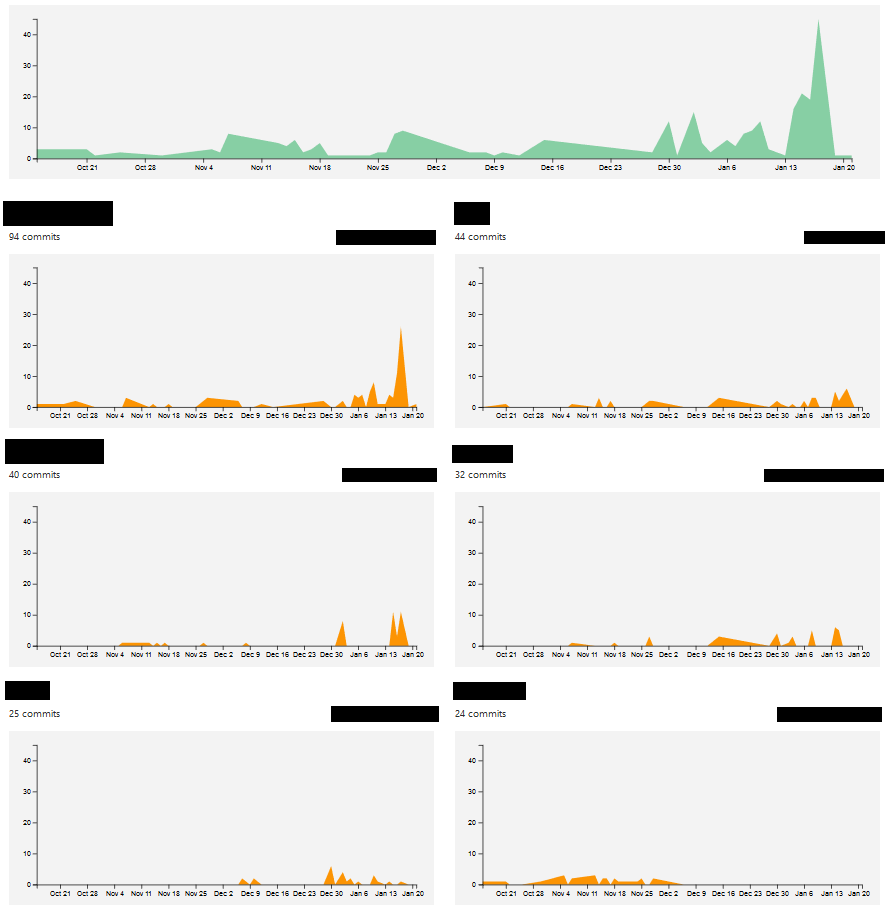
\includegraphics[scale=0.4]{slike/aktivnost.PNG} %veličina slike u odnosu na originalnu datoteku i pozicija slike
			\centering
			\caption{Primjer slike s potpisom}
			\label{fig:promjene}
		\end{figure}
		
		\begin{figure}[H]
			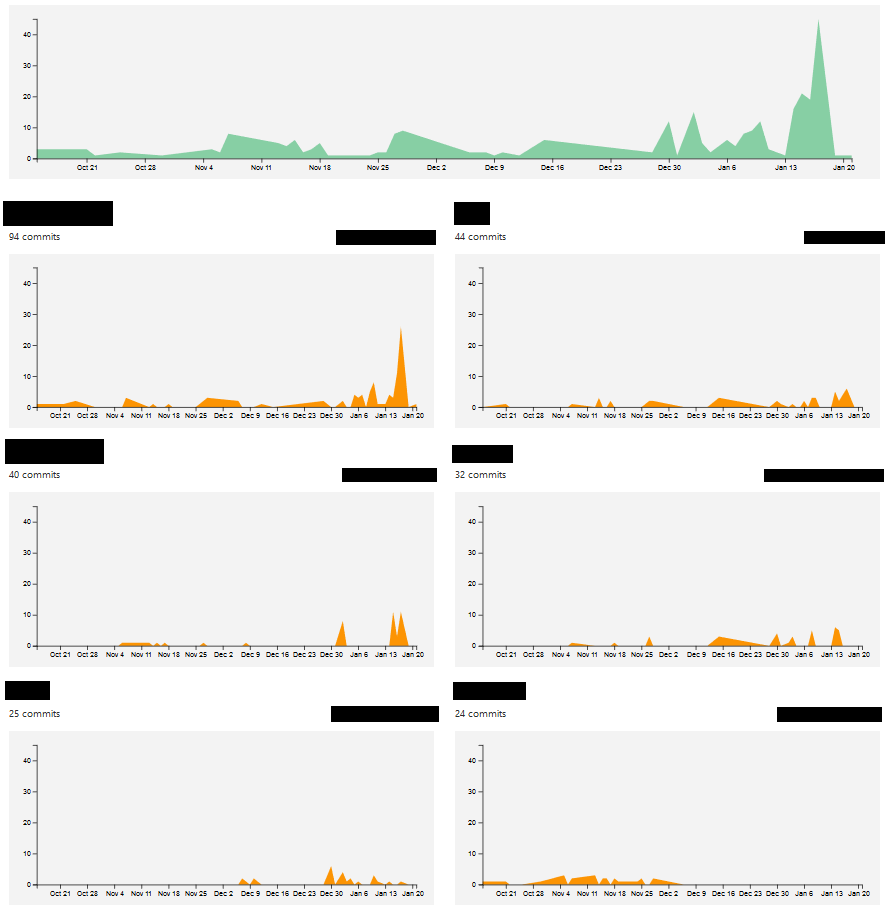
\includegraphics[width=\textwidth]{slike/aktivnost.PNG} %veličina u odnosu na širinu linije
			\caption{Primjer slike s potpisom 2}
			\label{fig:promjene2} %label mora biti drugaciji za svaku sliku
		\end{figure}
		
		Referenciranje slike \ref{fig:promjene2} u tekstu.
		
		\eject
		
	
	\chapter{Specifikacija programske potpore}
		
	\section{Funkcionalni zahtjevi}
			
			\noindent \textbf{Dionici:}
			
			\begin{packed_enum}
				
				\item Igrači
				\begin{packed_enum}
				    \item Igrač početnik
				    \item Napredni igrač
				\end{packed_enum}
				\item Kartograf				
				\item Administrator
				\item Razvojni tim
				
			\end{packed_enum}
			
			\noindent \textbf{Aktori i njihovi funkcionalni zahtjevi:}
			
			
			\begin{packed_enum}
				\item  \underbar{Neregistrirani/neprijavljeni korisnik (inicijator) može:}
				
				\begin{packed_enum}
					
					\item vidjeti stranicu dobrodošlice na kojoj se nalaze upute za korištenje aplikacije
					\item pregledati dostupne kartice na karti
					\item vidjeti globalnu statistiku odigranih borbi i sakupljenih lokacija te poredak svih igrača
					\item se registrirati u sustav, stvoriti novi korisnički račun za koji su mu potrebni korisničko ime, fotografija, lozinka i e-mail adresa
					
				\end{packed_enum}
			
				\item  \underbar{Igrač početnik (inicijator) može:}
				
				\begin{packed_enum}
					
					\item sakupljati lokacije, tj. kartice
					\item vidjeti popis ostalih aktivnih igrača koji se nalaze unutar 50 km i s njima ući u borbu
					
					\begin{packed_enum}
					    
					    \item odabir skupa karata s kojima će se boriti
					    
					\end{packed_enum}
					
					\item pristupiti pregledu profila igrača
					
					\begin{packed_enum}
					    
					    \item prikaz svih karata koje je igrač skupio
					    \item prikaz ranga na globalnoj ljestvici
					    \item prikaz statistike vezane uz zadnjih 10 borbi s drugim igračima
					    
					\end{packed_enum}
					
				\end{packed_enum}
				
			\item  \underbar{Napredni igrač (inicijator) može:}
				
				\begin{packed_enum}
					
					\item sakupljati lokacije, tj. kartice
					\item vidjeti popis ostalih aktivnih igrača koji se nalaze unutar 50 km i s njima ući u borbu
					
					\begin{packed_enum}
					    
					    \item odabir skupa karata s kojima će se boriti
					    
					\end{packed_enum}
					
					\item pristupiti pregledu profila igrača
					
					\begin{packed_enum}
					    
					    \item prikaz svih karata koje je igrač skupio
					    \item prikaz ranga na globalnoj ljestvici
					    \item prikaz statistike vezane uz zadnjih 10 borbi s drugim igračima
					    
					\end{packed_enum}
					
					\item prijaviti novu lokaciju (s potrebnim podacima) u čijoj se neposrednoj blizini nalazi
					
				\end{packed_enum}
				
			\item \underbar{Kartograf (inicijator) može:}
			
			    \begin{packed_enum}
			    
			        \item se registrirati za što su mu potrebni IBAN račun za uplatu i fotografija osobne iskaznice
			        \item nadopuniti bazu podatka s lokacijama koje su igrači prijavili
			        \item vidjeti prijave na karti
			        
			        \begin{packed_enum}
			            
			            \item odbijanje, potvrđivanje i uređivanje prijave
			            \item oznaka za potrebnu potvrdu s terena
			          
			        \end{packed_enum}
			        
			        \item označiti koje će prijave osobno provjeriti
			        
			    \end{packed_enum}
			    
		    \item \underbar{Administrator (inicijator) može:}
		    
		        \begin{packed_enum}
		            
		            \item vidjeti i uređivati popis svih registriranih korisnika i njihovih osobnih podataka
		            \item uređivati postojeće lokacije u igri
		            \item dodijeliti igračima privremeno isključenje iz igre
		            
		        \end{packed_enum}
		        
	        \item \underbar{Baza podataka (sudionik):}
		    
		        \begin{packed_enum}
		            
		            \item pohranjuje sve podatke o korisnicima i njihovim ovlastima
		            \item pohranjuje sve podatke o lokacijama
		            \item pohranjuje sve  podatke o provedenim borbama i izazovima
		            
		        \end{packed_enum}
		        
			\end{packed_enum}
			
			\eject 
			
			
				
			\subsection{Obrasci uporabe}
				
				
					\noindent \underbar{\textbf{UC1 - Registracija kao igrač}}
					\begin{packed_item}
	
						\item \textbf{Glavni sudionik: }Gost
						\item  \textbf{Cilj:} Stvoriti korisnički račun za pristup sustavu
						\item  \textbf{Sudionici:} Baza podataka
						\item  \textbf{Preduvjet:} -
						\item  \textbf{Opis osnovnog tijeka:}
						
						\item[] \begin{packed_enum}
	
							\item Gost odabire opciju za registraciju igrača
							\item Gost unosi potrebne korisničke podatke
							\item Gost dobiva e-mail kojim potvrđuje svoj račun

						\end{packed_enum}
						
						\item  \textbf{Opis mogućih odstupanja:}
						
						\item[] \begin{packed_item}
	
							\item[2.a] Odabir već zauzetog korisničkog imena i/ili e-maila, unos korisničkog podatka u nedozvoljenom formatu ili pružanje neispravnog e-maila
							\item[] \begin{packed_enum}
								
								\item Sustav obavještava korisnika o neuspjelom upisu i vraća ga na stranicu za registraciju
								\item Korisnik mijenja potrebne podatke te završava unos ili odustaje od registracije
								
							\end{packed_enum}
							
						\end{packed_item}
					\end{packed_item}
					
					\noindent \underbar{\textbf{UC2 - Registracija kao kartograf}}
					\begin{packed_item}
	
						\item \textbf{Glavni sudionik: }Gost
						\item  \textbf{Cilj:} Stvoriti korisnički račun za pristup sustavu
						\item  \textbf{Sudionici:} Baza podataka
						\item  \textbf{Preduvjet:} -
						\item  \textbf{Opis osnovnog tijeka:}
						
						\item[] \begin{packed_enum}
	
							\item Korisnik odabire opciju za registraciju kartografa
							\item Korisnik unosi potrebne korisničke podatke
							\item Korisnik dobiva e-amil kojim potvrđuje svoju prijavu
							\item Korisnika administratori potvrđuju kao kartografa

						\end{packed_enum}
						
						\item  \textbf{Opis mogućih odstupanja:}
						
						\item[] \begin{packed_item}
	
							\item[2.a] Odabir već zauzetog korisničkog imena i/ili e-maila, unos korisničkog podatka u nedozvoljenom formatu, pružanje neispravnog e-maila ili unos neispravnog IBAN-a
							\item[] \begin{packed_enum}
								
								\item Sustav obavještava korisnika o neuspjelom upisu i vraća ga na stranicu za registraciju
								\item Korisnik mijenja potrebne podatke te završava unos ili odustaje od registracije
								
							\end{packed_enum}
							
						\end{packed_item}
					\end{packed_item}
				
				    \noindent \underbar{\textbf{UC3 - Prijava u sustav}}
					\begin{packed_item}
	
						\item \textbf{Glavni sudionik:} Korisnik
						\item  \textbf{Cilj:} Dobiti pristup korisničkom sučelju
						\item  \textbf{Sudionici:} Baza podataka
						\item  \textbf{Preduvjet:} Registracija
						\item  \textbf{Opis osnovnog tijeka:}
						
						\item[] \begin{packed_enum}
	
							\item Unos korisničkog imena i lozinke
							\item Potvrda o ispravnosti unesenih podataka
							\item Pristup korisničkim funkcijama

						\end{packed_enum}
						
						\item  \textbf{Opis mogućih odstupanja:}
						
						\item[] \begin{packed_item}
	
							\item[2.a] Neispravno korisničko ime/e-mail/lozinka
							\item[] \begin{packed_enum}
								
								\item Sustav obavještava korisnika o neuspjelom upisu i vraća ga na stranicu za registraciju
								
							\end{packed_enum}
							
						\end{packed_item}
					\end{packed_item}
					
					\noindent \underbar{\textbf{UC4 - Pregled osobnih podataka}}
					\begin{packed_item}
	
						\item \textbf{Glavni sudionik: }Korisnik
						\item  \textbf{Cilj:} Pregledati osobne podatke i statistike
						\item  \textbf{Sudionici:} Baza podataka
						\item  \textbf{Preduvjet:} Korisnik je prijavljen
						\item  \textbf{Opis osnovnog tijeka:}
						
						\item[] \begin{packed_enum}
	
							\item Korisnik odabire opciju \textit{My Profile}
							\item Aplikacija prikazuje osobne podatke korisnika i njegovu statistiku

						\end{packed_enum}
						
					\end{packed_item}
					
					\noindent \underbar{\textbf{UC5 - Pregled profila drugih igrača}}
					\begin{packed_item}
	
						\item \textbf{Glavni sudionik: }Igrač
						\item  \textbf{Cilj:} Pregledati profil drugog igrača
						\item  \textbf{Sudionici:} Baza podataka
						\item  \textbf{Preduvjet:} Igrač je prijavljen
						\item  \textbf{Opis osnovnog tijeka:}
						
						\item[] \begin{packed_enum}
							\item Korisnik se nalazi na bilo kojoj stranici koja mu prikazuje korisničko ime drugog igrača
							\item Korisnik klikom na korisničko ime igrača zahtijeva pregled njegovog profila
							\item Korisniku se prikazuje javni profil odabranog korisnika
						\end{packed_enum}
					\end{packed_item}
					
					\noindent \underbar{\textbf{UC6 - Uređivanje vlastitih podataka}}
					\begin{packed_item}
	
						\item \textbf{Glavni sudionik: }Korisnik
						\item  \textbf{Cilj:} Urediti osobne podatke
						\item  \textbf{Sudionici:} Baza podataka
						\item  \textbf{Preduvjet:} Korisnik je prijavljen
						\item  \textbf{Opis osnovnog tijeka:}
						
						\item[] \begin{packed_enum}
	
							\item Korisnik odabire opciju za promjenu podataka
							\item Korisnik mijenja svoje osobne podatke
							\item Korisnik sprema promjene
							\item Baza podataka se ažurira

						\end{packed_enum}
						
						\item  \textbf{Opis mogućih odstupanja:}
						
						\item[] \begin{packed_item}
	
							\item[2.a] Korisnik promijeni svoje osobne podatke, ali ne odabere opciju \textit{Save changes}
							\item[] \begin{packed_enum}
								
								\item Sustav obavještava korisnika da nije spremio podatke prije izlaska iz prozora
								
							\end{packed_enum}
							
						\end{packed_item}
					\end{packed_item}
					
					\noindent \underbar{\textbf{UC7 - Brisanje korisničkog računa}}
					\begin{packed_item}
	
						\item \textbf{Glavni sudionik: }Korisnik
						\item  \textbf{Cilj:} Izbrisati svoj račun
						\item  \textbf{Sudionici:} Baza podataka
						\item  \textbf{Preduvjet:} Korisnik je prijavljen
						\item  \textbf{Opis osnovnog tijeka:}
						
						\item[] \begin{packed_enum}
	
							\item Korisnik pregledava osobne podatke
							\item Otvara se stranica s osobnim podacima korisnika
							\item Korisnik briše račun
							\item Korisnički račun se izbriše iz baze podataka
							\item Otvara se stranica za registraciju

						\end{packed_enum}
				
					\end{packed_item}
					
					\noindent \underbar{\textbf{UC8 - Skupljanje kartice}}
					\begin{packed_item}
	
						\item \textbf{Glavni sudionik: }Igrač
						\item  \textbf{Cilj:} Pokupiti karticu
						\item  \textbf{Sudionici:} Baza podataka
						\item  \textbf{Preduvjet:} Korisnik je prijavljen i nalazi se u neposrednoj blizini lokacije na kojoj je kartica
						\item  \textbf{Opis osnovnog tijeka:}
						
						\item[] \begin{packed_enum}
	
							\item Korisnik odabire karticu na karti
							\item Korisnik odabire opciju \textit{Collect}
							\item Kartica se nalazi na stranici \textit{My Profile -$>$ Inventory} 

						\end{packed_enum}
						
						\item  \textbf{Opis mogućih odstupanja:}
						
						\item[] \begin{packed_item}
	
							\item[2.a] Odabir kartice koju nije moguće pokupiti s korisnikove trenutne lokacije
							\item[] \begin{packed_enum}
								
								\item Sustav obavještava korisnika o neuspjelom sakupljanju kartice
								
							\end{packed_enum}
							
						\end{packed_item}
					\end{packed_item}
					
					\noindent \underbar{\textbf{UC9 - Pregled globalne statistike}}
					\begin{packed_item}
					
						\item \textbf{Glavni sudionik: }Korisnik
						\item  \textbf{Cilj:} Pregledati globalnu statistiku
						\item  \textbf{Sudionici:} Baza podataka
						\item  \textbf{Preduvjet:} Korisnik je prijavljen
						\item  \textbf{Opis osnovnog tijeka:}
						
						\item[] \begin{packed_enum}
	
							\item Korisnik odabire opciju \textit{Global stats} koja ga vodi na stranicu gdje dobiva uvid u globalnu statistiku

						\end{packed_enum}
						
					\end{packed_item}
				
				    \noindent \underbar{\textbf{UC10 - Pregled igrača u blizini}}
					\begin{packed_item}
	
						\item \textbf{Glavni sudionik: }Igrač
						\item  \textbf{Cilj:} Pregledati igrače u blizini
						\item  \textbf{Sudionici:} Baza podataka
						\item  \textbf{Preduvjet:} Igrač je prijavljen
						\item  \textbf{Opis osnovnog tijeka:}
						
						\item[] \begin{packed_enum}
	
							\item Korisnik odabire opciju prikaz liste najbližih igrača
						
						\end{packed_enum}
						
					\end{packed_item}
					
					\noindent \underbar{\textbf{UC11 - Izazivanje igrača}}
					\begin{packed_item}
	
						\item \textbf{Glavni sudionik: }Igrač
						\item  \textbf{Cilj:} Izazvati drugog igrača
						\item  \textbf{Sudionici:} Baza podataka
						\item  \textbf{Preduvjet:} Igrač je prijavljen i nalazi se unutar 50 km udaljenosti od drugog igrača
						\item  \textbf{Opis osnovnog tijeka:}
						
						\item[] \begin{packed_enum}
	
							\item Igrač odabire igrača kojeg želi izazvati
							\item Igrač šalje drugom igraču zahtjev za borbu

						\end{packed_enum}
						
					\end{packed_item}
					\pagebreak
					
					\noindent \underbar{\textbf{UC12 - Odgovor na izazov igrača}}
					\begin{packed_item}
	
						\item \textbf{Glavni sudionik: }Igrač
						\item  \textbf{Cilj:} Odgovoriti na izazov drugog igrača
						\item  \textbf{Sudionici:} Baza podataka
						\item  \textbf{Preduvjet:} Igrač je prijavljen
						\item  \textbf{Opis osnovnog tijeka:}
						
						\item[] \begin{packed_enum}
	
							\item Igrač dobiva obavijest o pristiglom izazovu
							\item Igrač označava \textit{Accept} ako prihvaća izazov ili \textit{Deny} ako odbija

						\end{packed_enum}
						
					\end{packed_item}
					
					\noindent \underbar{\textbf{UC13 - Izbor karata i borba}}
					\begin{packed_item}
	
						\item \textbf{Glavni sudionik: }Igrač
						\item  \textbf{Cilj:} Izabrati karte i boriti se s drugim igračem
						\item  \textbf{Sudionici:} Baza podataka
						\item  \textbf{Preduvjet:} Igrač je prijavljen i prihvatio je izazov ili je njegov izazov prihvaćen
						\item  \textbf{Opis osnovnog tijeka:}
						
						\item[] \begin{packed_enum}
	
							\item Korisnik odabire tri kartice među onima koje je prikupio
							\item Korisnik klikom na gumb \textit{Fight!} ulazi u borbu
							\item Korisniku se prikazuje ishod borbe i ažurirani broj njegovih bodova
						\end{packed_enum}
						
					\end{packed_item}
					
					\noindent \underbar{\textbf{UC14 - Prijava nove lokacije}}
					\begin{packed_item}
	
						\item \textbf{Glavni sudionik: }Napredni igrač
						\item  \textbf{Cilj:} Prijaviti novu lokaciju
						\item  \textbf{Sudionici:} Baza podataka
						\item  \textbf{Preduvjet:} Igrač je prijavljen i ima dovoljno visok \textit{ELO score}
						\item  \textbf{Opis osnovnog tijeka:}
						
						\item[] \begin{packed_enum}
	
							\item Igrač odabire opciju \textit{Add location}
							\item Igrač unosi naziv i opis te dodaje fotografiju

						\end{packed_enum}
						
						\item  \textbf{Opis mogućih odstupanja:}
						
						\item[] \begin{packed_item}
	
							\item[1.a] Igrač pokušava dodati lokaciju koja je previše udaljena od njegove trenutne lokacije
							\item[] \begin{packed_enum}
								
								\item Sustav obavještava igrača o neuspješnoj prijavi nove lokacije
								
							\end{packed_enum}
							
							\item[2.a] Nepotpun i/ili neispravan unos obaveznih podataka
							\item[] \begin{packed_enum}
								
								\item Sustav obavještava igrača o neuspješnom unosu obaveznih podataka i vraća ga na stranicu za prijavu nove lokacije
								
							\end{packed_enum}
							
						\end{packed_item}
					\end{packed_item}
					
					\noindent \underbar{\textbf{UC15 - Pregled lokacija koje čekaju pregled}}
					\begin{packed_item}
	
						\item \textbf{Glavni sudionik: }Igrač
						\item  \textbf{Cilj:} Pregledati vlastite predložene lokacije koje čekaju pregled kartografa.
						\item  \textbf{Sudionici:} Baza podataka
						\item  \textbf{Preduvjet:} Igrač je prijavljen
						\item  \textbf{Opis osnovnog tijeka:}
						
						\item[] \begin{packed_enum}
	
							\item Igrač se nalazi na stranici za predlaganje lokacija
							\item Igrač odabire filtar neodobrenih lokacija
							\item Igraču se na karti prikazuju vlastite predložene lokacije koje čekaju pregled.

						\end{packed_enum}
						
					\end{packed_item}
					
					\noindent \underbar{\textbf{UC16 - Pregled odobrenih lokacija}}
					\begin{packed_item}
	
						\item \textbf{Glavni sudionik: }Igrač
						\item  \textbf{Cilj:} Pregledati vlastite predložene lokacije koje su odobrene.
						\item  \textbf{Sudionici:} Baza podataka
						\item  \textbf{Preduvjet:} Igrač je prijavljen
						\item  \textbf{Opis osnovnog tijeka:}
						
						\item[] \begin{packed_enum}
	
							\item Igrač se nalazi na stranici za predlaganje lokacija
							\item Igrač odabire filtar odobrenih lokacija
							\item Igraču se na karti prikazuju vlastite predložene lokacije koje su prošle provjeru

						\end{packed_enum}
						
					\end{packed_item}
					
					\noindent \underbar{\textbf{UC17 - Pregled prijedloga lokacija}}
					\begin{packed_item}
	
						\item \textbf{Glavni sudionik: }Kartograf
						\item  \textbf{Cilj:} Pregledati predložene lokacije koje nisu odobrene.
						\item  \textbf{Sudionici:} Baza podataka
						\item  \textbf{Preduvjet:} Kartograf je prijavljen
						\item  \textbf{Opis osnovnog tijeka:}
						
						\item[] \begin{packed_enum}
	
							\item Kartograf se nalazi na početnoj stranici
							\item Kartograf odabire filtar neodobrenih lokacija
							\item Kartografu se na karti prikazuju predložene lokacije koje još nisu provjerene

						\end{packed_enum}
						
					\end{packed_item}
					\pagebreak
					
					\noindent \underbar{\textbf{UC18 - Uređivanje prijedloga lokacija}}
					\begin{packed_item}
	
						\item \textbf{Glavni sudionik: }Kartograf
						\item  \textbf{Cilj:} Urediti predloženu lokaciju koja nije odobrena.
						\item  \textbf{Sudionici:} Baza podataka
						\item  \textbf{Preduvjet:} Kartograf je prijavljen
						\item  \textbf{Opis osnovnog tijeka:}
						
						\item[] \begin{packed_enum}
	
							\item Kartograf se nalazi na početnoj stranici
							\item Kartograf odabire filtar neodobrenih lokacija
							\item Kartograf odabire lokaciju koju želi urediti
							\item Kartograf uređuje podatke u prijedlogu lokacije
							\item Kartograf sprema promjene
							\item Baza podataka se ažurira

						\end{packed_enum}
						
						\item  \textbf{Opis mogućih odstupanja:}
						
						\item[] \begin{packed_item}
	
							\item[2.a] Kartograf promijeni podatke o lokaciji, ali ne odabere opciju \textit{Save changes}
							\item[] \begin{packed_enum}
								
								\item Sustav obavještava kartografa da nije spremio podatke prije izlaska iz prozora
								
							\end{packed_enum}
							
						\end{packed_item}
					\end{packed_item}
					
					\noindent \underbar{\textbf{UC19 - Odobravanje prijedloga lokacija}}
					\begin{packed_item}
	
						\item \textbf{Glavni sudionik: }Kartograf
						\item  \textbf{Cilj:} Odobriti predloženu lokaciju
						\item  \textbf{Sudionici:} Baza podataka
						\item  \textbf{Preduvjet:} Kartograf je prijavljen
						\item  \textbf{Opis osnovnog tijeka:}
						
						\item[] \begin{packed_enum}
	
							\item Kartograf se nalazi na početnoj stranici
							\item Kartograf odabire filtar neodobrenih lokacija
							\item Kartografu se na karti prikazuju predložene lokacije koje još nisu odobrene
							\item Kartograf odabire lokaciju koju želi odobriti
							\item Kartograf odobrava lokaciju klikom na gumb \textit{Approve card}
							\item Baza podataka se ažurira

						\end{packed_enum}
						
					\end{packed_item}
					\pagebreak
					
					\noindent \underbar{\textbf{UC20 - Označavanje lokacije za provjeru}}
					\begin{packed_item}
	
						\item \textbf{Glavni sudionik: }Kartograf
						\item  \textbf{Cilj:} Označiti da je potrebna terenska provjera za predloženu lokaciju.
						\item  \textbf{Sudionici:} Baza podataka
						\item  \textbf{Preduvjet:} Kartograf je prijavljen
						\item  \textbf{Opis osnovnog tijeka:}
						
						\item[] \begin{packed_enum}
	
							\item Kartograf se nalazi na početnoj stranici
							\item Kartograf odabire filtar neodobrenih lokacija
							\item Kartografu se na karti prikazuju predložene lokacije koje još nisu odobrene
							\item Kartograf odabire lokaciju koju želi označiti za terensku provjeru
							\item Kartograf označava da je potrebna terenska provjera lokacije klikom na gumb \textit{Request on-site check}
							\item Baza podataka se ažurira

						\end{packed_enum}
						
					\end{packed_item}
					
					\noindent \underbar{\textbf{UC21 - Preuzimanje kartica za provjeru}}
					\begin{packed_item}
	
						\item \textbf{Glavni sudionik: }Kartograf
						\item  \textbf{Cilj:} Pregledati predložene lokacije koje trebaju terensku provjeru
						\item  \textbf{Sudionici:} Baza podataka
						\item  \textbf{Preduvjet:} Kartograf je prijavljen
						\item  \textbf{Opis osnovnog tijeka:}
						
						\item[] \begin{packed_enum}
	
							\item Kartograf se nalazi na stranici \textit{On-site approval}
							\item Kartograf odabire filtar koji će prikazati lokacije koje trebaju terensku provjeru
							\item Kartografu se na karti prikazuju predložene lokacije koje trebaju provjeru na terenu
							\item Kartograf klikom odabire lokaciju koju želi osobno obići, zatim klikne na gumb \textit{Add to my route}
							\item Baza podataka se ažurira

						\end{packed_enum}
						
					\end{packed_item}
					
					\noindent \underbar{\textbf{UC22 - Uklanjanje lokacija}} %Odustajanje od provjere?
					\begin{packed_item}
	
						\item \textbf{Glavni sudionik: }Kartograf
						\item  \textbf{Cilj:} Ukloniti lokaciju s vlastite liste za provjeru na terenu
						\item  \textbf{Sudionici:} Baza podataka
						\item  \textbf{Preduvjet:} Kartograf je prijavljen
						\item  \textbf{Opis osnovnog tijeka:}
						
						\item[] \begin{packed_enum}
	
							\item Kartograf se nalazi na stranici \textit{On-site approval}
							\item Kartograf odabire filtar koji će prikazati lokacije koje je dodao na vlastitu listu za provjeru na terenu
							\item Kartografu se na karti prikazuju njegove lokacije koje trebaju provjeru na terenu
							\item Kartograf klikom odabire lokaciju koju želi ukloniti iz rute, a uklanja ju klikom na gumb \textit{Remove}
							\item Baza podataka se ažurira

						\end{packed_enum}
						
					\end{packed_item}
					
					\noindent \underbar{\textbf{UC23 - Generiranje rute}}
					\begin{packed_item}
	
						\item \textbf{Glavni sudionik: }Kartograf
						\item  \textbf{Cilj:} Generirati najkraću rutu za obilazak odabranih lokacija
UC						\item  \textbf{Sudionici:} Baza podataka, OSRM servis
						\item  \textbf{Preduvjet:} Kartograf je prijavljen
						\item  \textbf{Opis osnovnog tijeka:}
						
						\item[] \begin{packed_enum}
	
							\item Kartograf se nalazi na stranici \textit{On-site approval}
							\item Kartografu se na karti prikazuju predložene lokacije koje trebaju provjeru na terenu
							\item Kartograf odabire filtre po želji - može prikazati lokacije koje je dodao na vlastitu listu za provjeru na terenu i/ili lokacije koje trebaju terensku provjeru, ali ih nitko nije zadužio
							\item Kartograf izražava zahtjev za generiranjem rute koja će obići sve odabrane lokacije klikom na gumb \textit{Generate route}
							\item Sustav rješava problem trgovačkog putnika putem vanjskog servisa i prikazuje kartografu generiranu rutu
							
						\end{packed_enum}
						
					\end{packed_item}
					
					\noindent \underbar{\textbf{UC24 - Odobravanje lokacije}}
					\begin{packed_item}
	
						\item \textbf{Glavni sudionik: }Kartograf
						\item  \textbf{Cilj:} Odobriti lokaciju s vlastite liste za terensku provjeru
						\item  \textbf{Sudionici:} Baza podataka
						\item  \textbf{Preduvjet:} Kartograf je prijavljen
						\item  \textbf{Opis osnovnog tijeka:}
						
						\item[] \begin{packed_enum}
	
							\item Kartograf se nalazi na stranici \textit{On-site approval}
							\item Kartografu se ispod karte prikazuje lista lokacija koje je dodao na vlastitu listu za provjeru na terenu
							\item Kartograf pojedinu lokaciju odobrava klikom na gumb \textit{Approve}
							\item Baza podataka se ažurira
							
						\end{packed_enum}
						
					\end{packed_item}
					
					\noindent \underbar{\textbf{UC25 - Pregled osobno odobrenih lokacija}}
					\begin{packed_item}
	
						\item \textbf{Glavni sudionik: }Kartograf
						\item  \textbf{Cilj:} Kartograf želi pregledati popis lokacija koje je do sada odobrio
						\item  \textbf{Sudionici:} Baza podataka
						\item  \textbf{Preduvjet:} Kartograf je prijavljen
						\item  \textbf{Opis osnovnog tijeka:}
						
						\item[] \begin{packed_enum}
	
							\item Kartograf se nalazi na stranici \textit{My profile}
							\item Kartografu se na njegovom profilu prikazuje lista svih lokacija koje je odobrio
							
						\end{packed_enum}
						
					\end{packed_item}
					
					\noindent \underbar{\textbf{UC26 - Pregled podataka svih korisnika}}
					\begin{packed_item}
	
						\item \textbf{Glavni sudionik: }Administrator
						\item  \textbf{Cilj:} Dobiti uvid u osobne podatke svih korisnika
						\item  \textbf{Sudionici:} Baza podataka
						\item  \textbf{Preduvjet:} Administrator je prijavljen
						\item  \textbf{Opis osnovnog tijeka:}
						
						\item[] \begin{packed_enum}
	
							\item Administrator se nalazi na stranici \textit{All users}
							\item Administrator vidi popis svih korisnika i klikom na korisničko ime pojedinog korisnika biva odveden na stranicu gdje dobiva uvid u njegove osobne podatke
							
						\end{packed_enum}
						
					\end{packed_item}
					
					\noindent \underbar{\textbf{UC27 - Uređivanje podataka korisnika}}
					\begin{packed_item}
	
						\item \textbf{Glavni sudionik: }Administrator
						\item  \textbf{Cilj:} Urediti osobne podatke nekog korisnika
						\item  \textbf{Sudionici:} Baza podataka
						\item  \textbf{Preduvjet:} Administrator je prijavljen
						\item  \textbf{Opis osnovnog tijeka:}
						
						\item[] \begin{packed_enum}
	
							\item Administrator se nalazi na stranici \textit{All users}
							\item Administrator vidi popis svih korisnika i klikom na gumb za uređivanje pored korisničkog imena pojedinog korisnika biva odveden na stranicu gdje dobiva mogućnost izmjene njegovih osobnih podataka
							
						\end{packed_enum}
						
						\pagebreak
						\item  \textbf{Opis mogućih odstupanja:}
						\item[] \begin{packed_item}
	
							\item[2.a] Administrator na gumb iste funkcionalnosti može kliknuti na stranici gdje pregledava osobne podatke nekog korisnika (UC26)
							\item[] \begin{packed_enum}
								
								\item Sustav odvodi administratora na stranicu za izmjenu osobnih podataka
								
							\end{packed_enum}
						\end{packed_item}
					\end{packed_item}
					
					\noindent \underbar{\textbf{UC28 - Privremeno isključenje korisnika}}
					\begin{packed_item}
	
						\item \textbf{Glavni sudionik: }Administrator
						\item  \textbf{Cilj:} Privremeno onemogućiti pristup aplikaciji za nekog korisnika
						\item  \textbf{Sudionici:} Baza podataka
						\item  \textbf{Preduvjet:} Administrator je prijavljen
						\item  \textbf{Opis osnovnog tijeka:}
						
						\item[] \begin{packed_enum}
	
							\item Administrator se nalazi na stranici \textit{All users}
							\item Administrator vidi popis svih korisnika i klikom na gumb za isključenje isključuje korisnika na konačan vremenski period
							
						\end{packed_enum}
						
					\end{packed_item}
					
					\noindent \underbar{\textbf{UC29 - Pregled svih lokacija}}
					\begin{packed_item}
	
						\item \textbf{Glavni sudionik: }Administrator
						\item  \textbf{Cilj:} Dobiti uvid u podatke o svim lokacijama						\item  \textbf{Sudionici:} Baza podataka
						\item  \textbf{Preduvjet:} Administrator je prijavljen
						\item  \textbf{Opis osnovnog tijeka:}
						
						\item[] \begin{packed_enum}
	
							\item Administrator se nalazi na stranici \textit{All cards}
							\item Administrator vidi popis svih kartica i klikom na pojedinu biva odveden na stranicu gdje dobiva uvid u podatke o njoj
							
						\end{packed_enum}
						
					\end{packed_item}
					
					\noindent \underbar{\textbf{UC30 - Uređivanje podataka lokacije}}
					\begin{packed_item}
	
						\item \textbf{Glavni sudionik: }Administrator
						\item  \textbf{Cilj:} Urediti podatke neke lokacije
						\item  \textbf{Sudionici:} Baza podataka
						\item  \textbf{Preduvjet:} Administrator je prijavljen
						\item  \textbf{Opis osnovnog tijeka:}
						
						\item[] \begin{packed_enum}
	
							\item Administrator se nalazi na stranici \textit{All cards}
							\item Administrator vidi popis svih lokacija i klikom na gumb za uređivanje pored pojedine kartice biva odveden na stranicu gdje dobiva mogućnost izmjene podataka o lokaciji
							
						\end{packed_enum}
						
						\item  \textbf{Opis mogućih odstupanja:}
						\item[] \begin{packed_item}
	
							\item[2.a] Administrator na gumb iste funkcionalnosti može kliknuti na stranici gdje pregledava podatke o lokaciji (UC29)
							\item[] \begin{packed_enum}
								
								\item Sustav odvodi administratora na stranicu za izmjenu podataka o lokaciji
								
							\end{packed_enum}
						\end{packed_item}
					\end{packed_item}
					
					\noindent \underbar{\textbf{UC31 - Pregled neodobrenih kartografa}}
					\begin{packed_item}
	
						\item \textbf{Glavni sudionik: }Administrator
						\item  \textbf{Cilj:} Dobiti uvid u neodobrene registracije kartografa
						\item  \textbf{Sudionici:} Baza podataka
						\item  \textbf{Preduvjet:} Administrator je prijavljen
						\item  \textbf{Opis osnovnog tijeka:}
						
						\item[] \begin{packed_enum}
	
							\item Administrator se nalazi na stranici \textit{Cartograph approvals}
							\item Administrator vidi popis svih neodobrenih registracija kartografa i klikom na pojedinu biva odveden na stranicu gdje dobiva uvid u podatke koje je kartograf predao u prijavi
							
						\end{packed_enum}
						
					\end{packed_item}
					
					\noindent \underbar{\textbf{UC32 - Odobravanje kartografa}}
					\begin{packed_item}
	
						\item \textbf{Glavni sudionik: }Administrator
						\item  \textbf{Cilj:} Odobriti registraciju kartografa
						\item  \textbf{Sudionici:} Baza podataka
						\item  \textbf{Preduvjet:} Administrator je prijavljen
						\item  \textbf{Opis osnovnog tijeka:}
						
						\item[] \begin{packed_enum}
	
							\item Administrator se nalazi na na kojoj ima uvid u podatke koje je kartograf predao u prijavi (UC31)
							\item Klikom na gumb \textit{Approve} administrator odobrava registraciju kartografa
							
						\end{packed_enum}
						
					\end{packed_item}
					
					
				\subsubsection{Dijagrami obrazaca uporabe}
				
				\begin{figure}[H]
        			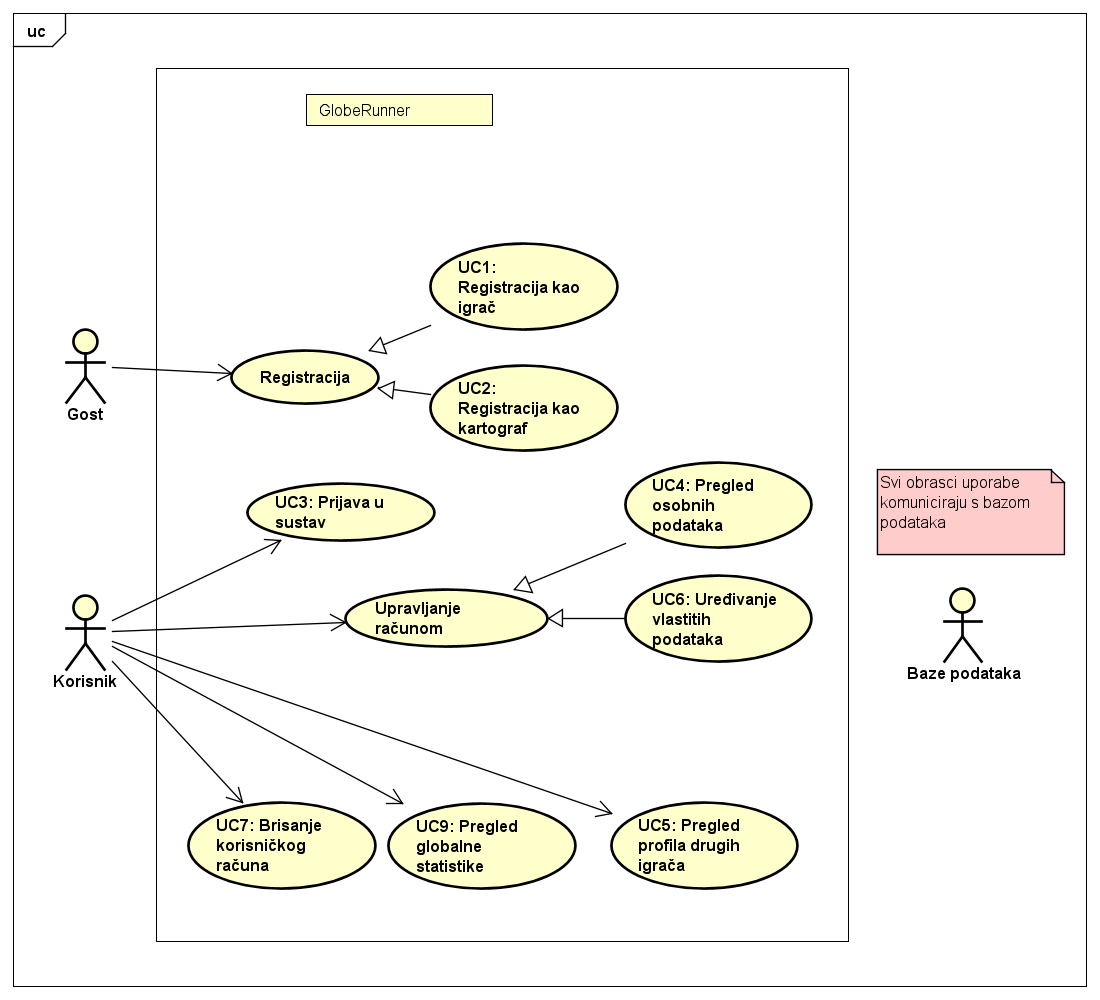
\includegraphics[scale=0.5]{slike/UCDiagrami/korisnik.png} %veličina slike u odnosu na originalnu datoteku i pozicija slike
        			\centering
        			\caption{Dijagram obrasca uporabe, funkcionalnost gosta i korisnika}
        			\label{fig:promjene}
        		\end{figure}
					
				\begin{figure}[H]
        			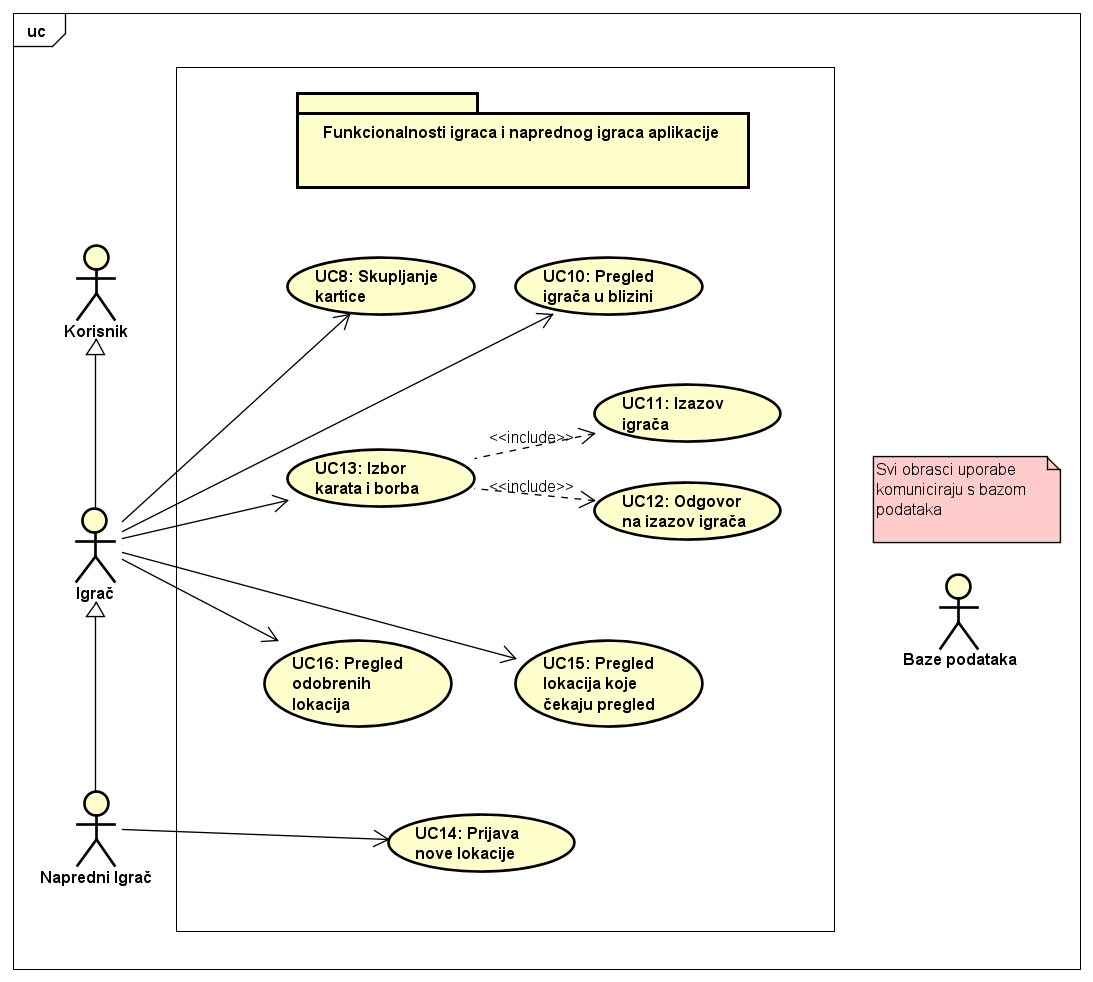
\includegraphics[scale=0.5]{slike/UCDiagrami/igrac.png} %veličina slike u odnosu na originalnu datoteku i pozicija slike
        			\centering
        			\caption{Dijagram obrasca uporabe, funkcionalnost igrača i naprednog igrača}
        			\label{fig:promjene}
        		\end{figure}
					
				\begin{figure}[H]
        			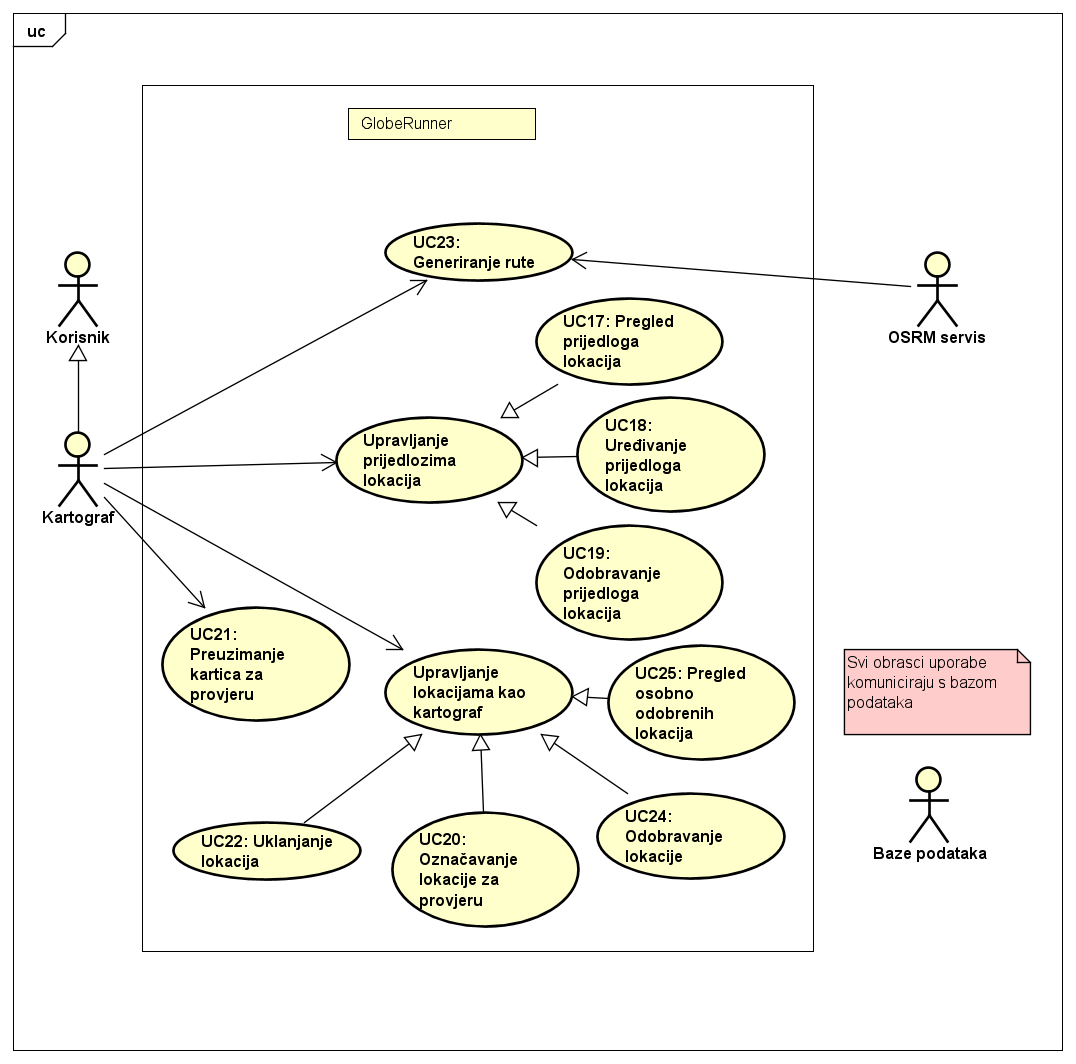
\includegraphics[scale=0.5]{slike/UCDiagrami/kartograf.png} %veličina slike u odnosu na originalnu datoteku i pozicija slike
        			\centering
        			\caption{Dijagram obrasca uporabe, funkcionalnost kartografa}
        			\label{fig:promjene}
        		\end{figure}
					
				\begin{figure}[H]
        			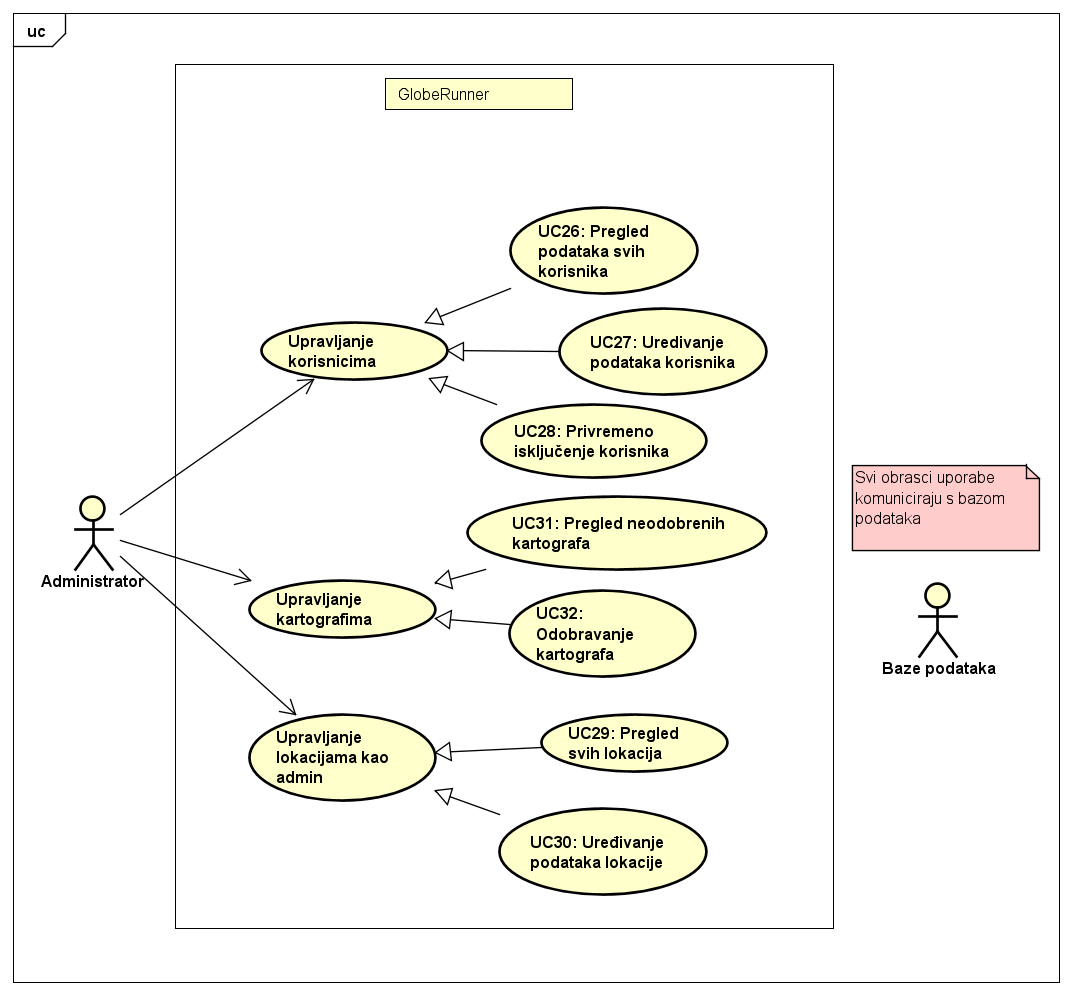
\includegraphics[scale=0.5]{slike/UCDiagrami/admin.png} %veličina slike u odnosu na originalnu datoteku i pozicija slike
        			\centering
        			\caption{Dijagram obrasca uporabe, funkcionalnost admina}
        			\label{fig:promjene}
        		\end{figure}
				
			\pagebreak
			\subsection{Sekvencijski dijagrami}
				
				\subsubsection{Obrazac uporabe UC14 - Prijava nove lokacije}
				
				Napredni igrač šalje zahtjev za dodavanje kartice te mu poslužitelj prikazuje sučelje za unos podataka o novoj kartici/lokaciji. Napredni igrač unosi sve podatke o kartici koju želi dodati te sprema provjere. Poslužitelj tada provjerava ispravnost unesenih podataka te ih, u slučaju uspješne validacije, sprema u bazu. Nakon toga, poslužitelj naprednom igraču ispisuje poruku o uspješnom dodavanju nove kartice/lokacije.
				
				\begin{figure}[H]
        			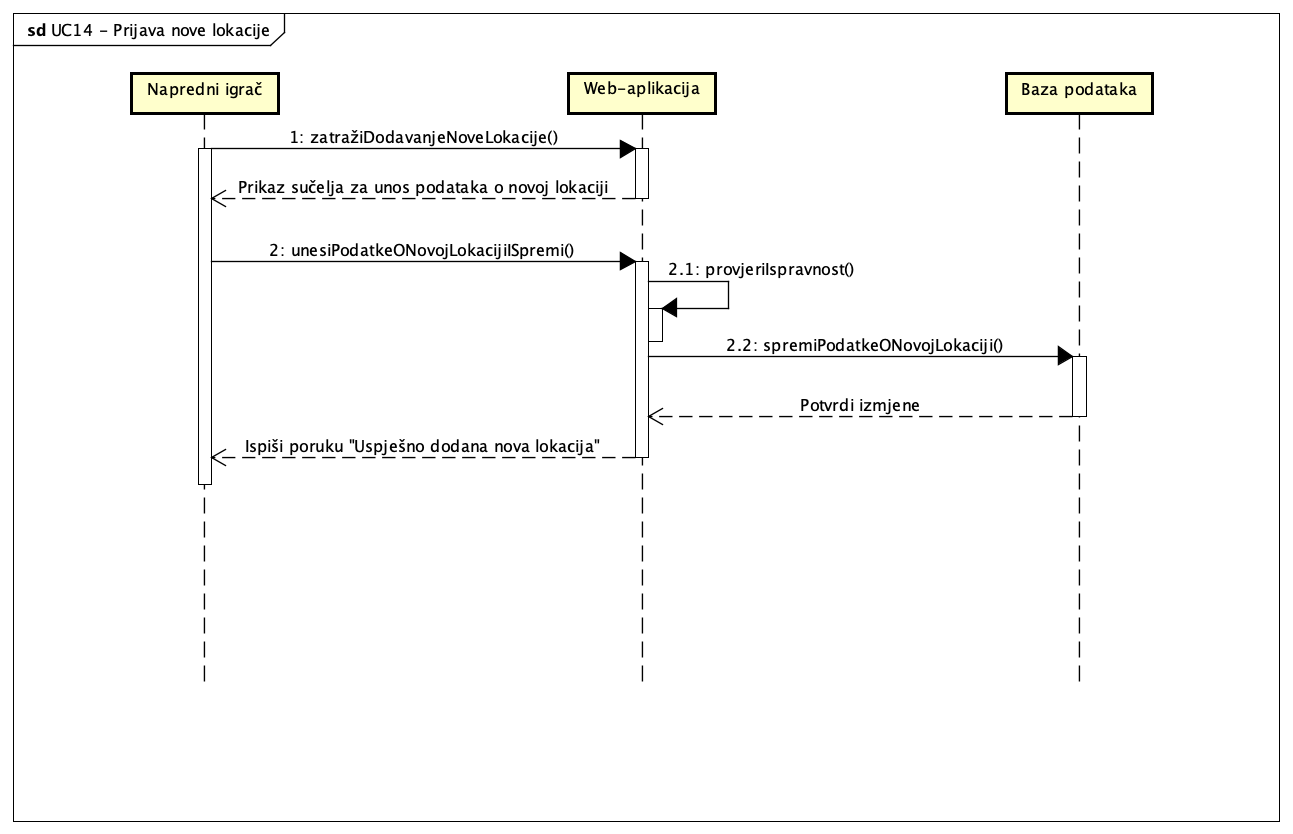
\includegraphics[scale=0.4]{slike/Sekvencijski dijagrami/UC14 - Prijava nove lokacije.png}
        			\centering
        			\caption{Sekvencijski dijagram za UC14}
        			\label{fig:promjene}
        		\end{figure}
				
				\pagebreak
				\subsubsection{Obrasci uporabe UC17 - Pregled prijedloga i UC18 - Uređivanje prijedloga}
				
				Kartograf šalje zahtjev za prikaz neodobrenih lokacija. Poslužitelj dohvaća neodobrene lokacije iz baze te ih prikazuje kartografu. Kartograf šalje zahtjev za izmjenu podataka o odabranoj lokaciji/kartici. Poslužitelj prikazuje kartografu sučelje za uređivanje postojećih podataka o neodobrenoj lokaciji. Kartograf unosi izmjene u prikazano sučelje. Ako kartograf pokuša zatvoriti prozor prije spremanja unesenih izmjena, poslužitelj ga upozorava da promjene nisu spremljene. Tada kartograf može odabrati svejedno zatvoriti prozor ili spremiti promjene. Ako odabere zatvoriti prozor prije spremanja, unesene izmjene neće biti spremljene u bazu. Ako odabere spremiti promjene, poslužitelj unesene podatke o lokaciji sprema u bazu te ispisuje poruku o uspješnoj izmjeni podataka.
				
				\begin{figure}[H]
        			\includegraphics[scale=0.3]{slike/Sekvencijski dijagrami/UC17 - Pregled prijedloga, UC18 - Uređivanje prijedloga.png}
        			\centering
        			\caption{Sekvencijski dijagram za UC17, UC18}
        			\label{fig:promjene}
        		\end{figure}
        		
        		\pagebreak
        		\subsubsection{Obrasci uporabe UC21 - Preuzimanje kartice za provjeru i UC23 - Generiranje rute}
        		
        		Kartograf šalje zahtjev za prikaz kartica koje trebaju terensku provjeru. Poslužitelj dohvaća kartice koje trebaju terensku provjeru iz baze te ih prikazuje kartografu. Kartograf šalje zahtjev za preuzimanjem kartice za provjeru. Poslužitelj u bazu podataka bilježi da je kartica preuzeta za provjeru te bilježi koji kartograf ju je preuzeo. Kartograf prije generiranja rute još jednom šalje zahtjev za prikaz neodobrenih lokacija. Poslužitelj ih dohvaća iz baze podataka te prikazuje kartografu. Kartograf šalje zahtjev za generiranje rute. Poslužitelj iz baze dohvaća kartice koje je taj kartograf preuzeo za provjeru te ih šalje OSRM servisu i zahtjeva generiranje rute. OSRM servis poslužitelju vraća generiranu rutu, a poslužitelj ju prikazuje kartografu.
				
				\begin{figure}[H]
        			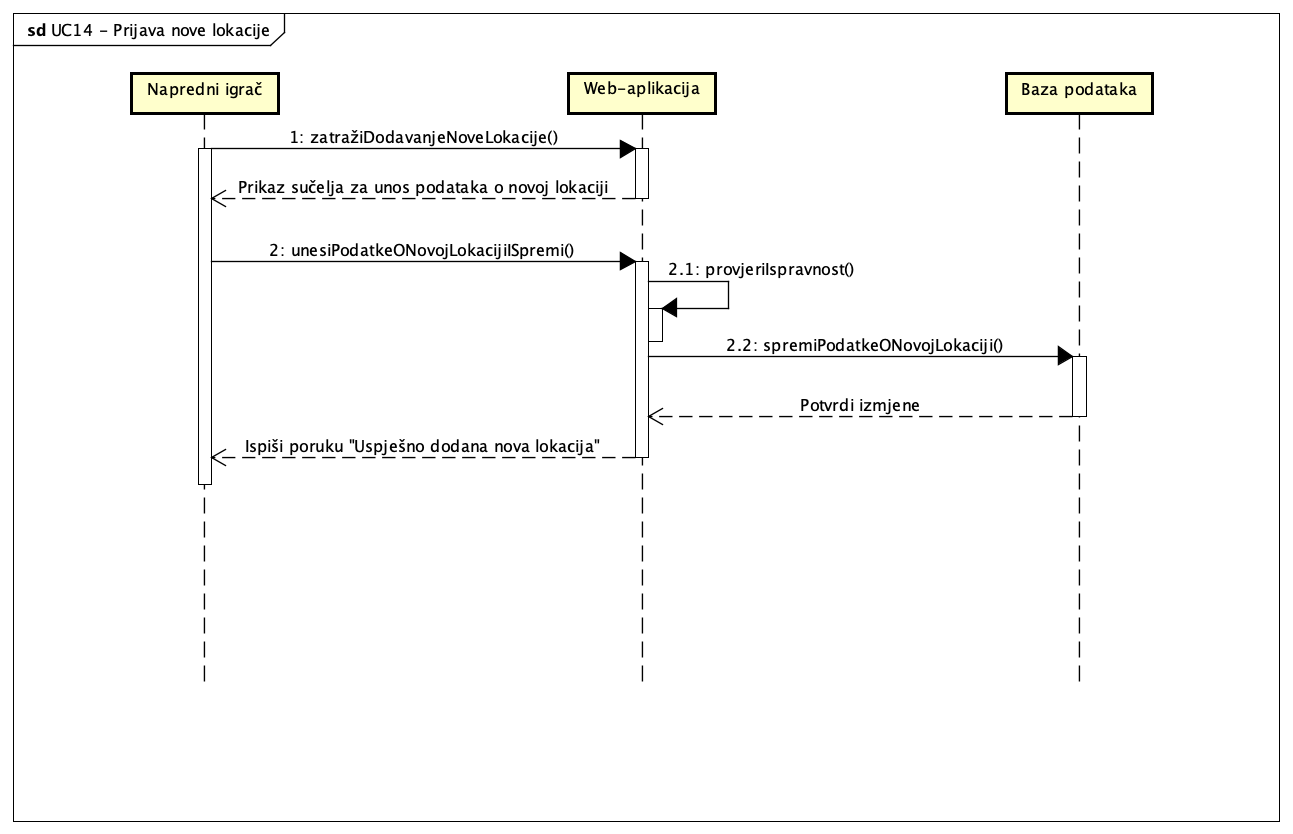
\includegraphics[scale=0.4]{slike/Sekvencijski dijagrami/UC14 - Prijava nove lokacije.png}
        			\centering
        			\caption{Sekvencijski dijagram za UC21, UC23}
        			\label{fig:promjene}
        		\end{figure}
	    \pagebreak
		\section{Ostali zahtjevi}
		\begin{packed_item}
		    \item Sustav treba omogućiti rad više korisnika u stvarnom vremenu
			\item Korisničko sučelje i sustav moraju podržavati hrvatsku abecedu (dijakritičke znakove) pri unosu i prikazu tekstualnog sadržaja
			\item Izvršavanje dijela programa u kojem se pristupa bazi podataka ne smije trajati duže od nekoliko sekundi
			\item Sustav treba biti implementiran kao web aplikacija koristeći objektno-orijentirane jezike
			\item Neispravno korištenje korisničkog sučelja ne smije narušiti funkcionalnost i rad sustava
			\item Sustav treba biti jednostavan za korištenje, korisnici se moraju znati koristiti sučeljem bez opširnih uputa
			\item Nadogradnja sustava ne smije narušavati postojeće funkcionalnosti sustava
			\item Sustav kao valutu koristi EURO
			\item Veza s bazom podataka mora biti kvalitetno zaštićena, brza i otporna na vanjske greške
			\item Pristup sustavu mora biti omogućen iz javne mreže pomoću HTTPS
			\item Rukovanje osobnim podatcima treba biti usklađeno s važećim direktivama
			\item Sustav treba koristiti GPS za pozicioniranje igrača i kartica na karti
			\item Sustav treba koristiti OSRM servis za rješavanje problema trgovačkog putnika
			
		\end{packed_item}
	\chapter{Arhitektura i dizajn sustava}
		
		\textbf{\textit{dio 1. revizije}}\\

		\textit{ Potrebno je opisati stil arhitekture te identificirati: podsustave, preslikavanje na radnu platformu, spremišta podataka, mrežne protokole, globalni upravljački tok i sklopovsko-programske zahtjeve. Po točkama razraditi i popratiti odgovarajućim skicama:}
	\begin{itemize}
		\item 	\textit{izbor arhitekture temeljem principa oblikovanja pokazanih na predavanjima (objasniti zašto ste baš odabrali takvu arhitekturu)}
		\item 	\textit{organizaciju sustava s najviše razine apstrakcije (npr. klijent-poslužitelj, baza podataka, datotečni sustav, grafičko sučelje)}
		\item 	\textit{organizaciju aplikacije (npr. slojevi frontend i backend, MVC arhitektura) }		
	\end{itemize}

	
		

		

				
		\section{Baza podataka}
			
			\textbf{\textit{dio 1. revizije}}\\
			
		\textit{Potrebno je opisati koju vrstu i implementaciju baze podataka ste odabrali, glavne komponente od kojih se sastoji i slično.}
		
			\subsection{Opis tablica}
			

				\textit{Svaku tablicu je potrebno opisati po zadanom predlošku. Lijevo se nalazi točno ime varijable u bazi podataka, u sredini se nalazi tip podataka, a desno se nalazi opis varijable. Svjetlozelenom bojom označite primarni ključ. Svjetlo plavom označite strani ključ}
				
				
				\begin{longtblr}[
					label=none,
					entry=none
					]{
						width = \textwidth,
						colspec={|X[6,l]|X[6, l]|X[20, l]|}, 
						rowhead = 1,
					} %definicija širine tablice, širine stupaca, poravnanje i broja redaka naslova tablice
					\hline \multicolumn{3}{|c|}{\textbf{korisnik - ime tablice}}	 \\ \hline[3pt]
					\SetCell{LightGreen}IDKorisnik & INT	&  	Lorem ipsum dolor sit amet, consectetur adipiscing elit, sed do eiusmod  	\\ \hline
					korisnickoIme	& VARCHAR &   	\\ \hline 
					email & VARCHAR &   \\ \hline 
					ime & VARCHAR	&  		\\ \hline 
					\SetCell{LightBlue} primjer	& VARCHAR &   	\\ \hline 
				\end{longtblr}
				
				
			
			\subsection{Dijagram baze podataka}
				\textit{ U ovom potpoglavlju potrebno je umetnuti dijagram baze podataka. Primarni i strani ključevi moraju biti označeni, a tablice povezane. Bazu podataka je potrebno normalizirati. Podsjetite se kolegija "Baze podataka".}
			
			\eject
			
			
		\section{Dijagram razreda}
		
			\textit{Potrebno je priložiti dijagram razreda s pripadajućim opisom. Zbog preglednosti je moguće dijagram razlomiti na više njih, ali moraju biti grupirani prema sličnim razinama apstrakcije i srodnim funkcionalnostima.}\\
			
			\textbf{\textit{dio 1. revizije}}\\
			
			\textit{Prilikom prve predaje projekta, potrebno je priložiti potpuno razrađen dijagram razreda vezan uz \textbf{generičku funkcionalnost} sustava. Ostale funkcionalnosti trebaju biti idejno razrađene u dijagramu sa sljedećim komponentama: nazivi razreda, nazivi metoda i vrste pristupa metodama (npr. javni, zaštićeni), nazivi atributa razreda, veze i odnosi između razreda.}\\
			
			\textbf{\textit{dio 2. revizije}}\\			
			
			\textit{Prilikom druge predaje projekta dijagram razreda i opisi moraju odgovarati stvarnom stanju implementacije}
			
			
			
			\eject
		
		\section{Dijagram stanja}
			
			
			\textbf{\textit{dio 2. revizije}}\\
			
			\textit{Potrebno je priložiti dijagram stanja i opisati ga. Dovoljan je jedan dijagram stanja koji prikazuje \textbf{značajan dio funkcionalnosti} sustava. Na primjer, stanja korisničkog sučelja i tijek korištenja neke ključne funkcionalnosti jesu značajan dio sustava, a registracija i prijava nisu. }
			
			
			\eject 
		
		\section{Dijagram aktivnosti}
			
			\textbf{\textit{dio 2. revizije}}\\
			
			 \textit{Potrebno je priložiti dijagram aktivnosti s pripadajućim opisom. Dijagram aktivnosti treba prikazivati značajan dio sustava.}
			
			\eject
		\section{Dijagram komponenti}
		
			\textbf{\textit{dio 2. revizije}}\\
		
			 \textit{Potrebno je priložiti dijagram komponenti s pripadajućim opisom. Dijagram komponenti treba prikazivati strukturu cijele aplikacije.}
	\chapter{Implementacija i korisničko sučelje}
		
		
		\section{Korištene tehnologije i alati}
		
			\textbf{\textit{dio 2. revizije}}
			
			 \textit{Detaljno navesti sve tehnologije i alate koji su primijenjeni pri izradi dokumentacije i aplikacije. Ukratko ih opisati, te navesti njihovo značenje i mjesto primjene. Za svaki navedeni alat i tehnologiju je potrebno \textbf{navesti internet poveznicu} gdje se mogu preuzeti ili više saznati o njima}.
			
			
			\eject 
		
	
		\section{Ispitivanje programskog rješenja}
			
			\textbf{\textit{dio 2. revizije}}\\
			
			 \textit{U ovom poglavlju je potrebno opisati provedbu ispitivanja implementiranih funkcionalnosti na razini komponenti i na razini cijelog sustava s prikazom odabranih ispitnih slučajeva. Studenti trebaju ispitati temeljnu funkcionalnost i rubne uvjete.}
	
			
			\subsection{Ispitivanje komponenti}
			\textit{Potrebno je provesti ispitivanje jedinica (engl. unit testing) nad razredima koji implementiraju temeljne funkcionalnosti. Razraditi \textbf{minimalno 6 ispitnih slučajeva} u kojima će se ispitati redovni slučajevi, rubni uvjeti te izazivanje pogreške (engl. exception throwing). Poželjno je stvoriti i ispitni slučaj koji koristi funkcionalnosti koje nisu implementirane. Potrebno je priložiti izvorni kôd svih ispitnih slučajeva te prikaz rezultata izvođenja ispita u razvojnom okruženju (prolaz/pad ispita). }
			
			
			
			\subsection{Ispitivanje sustava}
			
			 \textit{Potrebno je provesti i opisati ispitivanje sustava koristeći radni okvir Selenium\footnote{\url{https://www.seleniumhq.org/}}. Razraditi \textbf{minimalno 4 ispitna slučaja} u kojima će se ispitati redovni slučajevi, rubni uvjeti te poziv funkcionalnosti koja nije implementirana/izaziva pogrešku kako bi se vidjelo na koji način sustav reagira kada nešto nije u potpunosti ostvareno. Ispitni slučaj se treba sastojati od ulaza (npr. korisničko ime i lozinka), očekivanog izlaza ili rezultata, koraka ispitivanja i dobivenog izlaza ili rezultata.\\ }
			 
			 \textit{Izradu ispitnih slučajeva pomoću radnog okvira Selenium moguće je provesti pomoću jednog od sljedeća dva alata:}
			 \begin{itemize}
			 	\item \textit{dodatak za preglednik \textbf{Selenium IDE} - snimanje korisnikovih akcija radi automatskog ponavljanja ispita	}
			 	\item \textit{\textbf{Selenium WebDriver} - podrška za pisanje ispita u jezicima Java, C\#, PHP koristeći posebno programsko sučelje.}
			 \end{itemize}
		 	\textit{Detalji o korištenju alata Selenium bit će prikazani na posebnom predavanju tijekom semestra.}
			
			\eject 
		
		
		\section{Dijagram razmještaja}
			
			\textbf{\textit{dio 2. revizije}}
			
			 \textit{Potrebno je umetnuti \textbf{specifikacijski} dijagram razmještaja i opisati ga. Moguće je umjesto specifikacijskog dijagrama razmještaja umetnuti dijagram razmještaja instanci, pod uvjetom da taj dijagram bolje opisuje neki važniji dio sustava.}
			
			\eject 
		
		\section{Upute za puštanje u pogon}
		
			\textbf{\textit{dio 2. revizije}}\\
		
			 \textit{U ovom poglavlju potrebno je dati upute za puštanje u pogon (engl. deployment) ostvarene aplikacije. Na primjer, za web aplikacije, opisati postupak kojim se od izvornog kôda dolazi do potpuno postavljene baze podataka i poslužitelja koji odgovara na upite korisnika. Za mobilnu aplikaciju, postupak kojim se aplikacija izgradi, te postavi na neku od trgovina. Za stolnu (engl. desktop) aplikaciju, postupak kojim se aplikacija instalira na računalo. Ukoliko mobilne i stolne aplikacije komuniciraju s poslužiteljem i/ili bazom podataka, opisati i postupak njihovog postavljanja. Pri izradi uputa preporučuje se \textbf{naglasiti korake instalacije uporabom natuknica} te koristiti što je više moguće \textbf{slike ekrana} (engl. screenshots) kako bi upute bile jasne i jednostavne za slijediti.}
			
			
			 \textit{Dovršenu aplikaciju potrebno je pokrenuti na javno dostupnom poslužitelju. Studentima se preporuča korištenje neke od sljedećih besplatnih usluga: \href{https://aws.amazon.com/}{Amazon AWS}, \href{https://azure.microsoft.com/en-us/}{Microsoft Azure} ili \href{https://www.heroku.com/}{Heroku}. Mobilne aplikacije trebaju biti objavljene na F-Droid, Google Play ili Amazon App trgovini.}
			
			
			\eject 
	\chapter{Zaključak i budući rad}
		 
		 Naša je grupa imala zadatak razviti web aplikaciju koja funkcionira kao online igra u kojoj igrači prikupljaju kartice i s njima ulaze u bitke s obližnjim igračima, dok najbolji među njima mogu predlagati nove lokacije koje kartografi pak pregledavaju, uređuju i odobravaju, a administratori sve to nadziru uz potpunu kontrolu nad korisnicima i lokacijama. Na ovom smo projektu radili 10 tjedana i uspješno smo implementirali tražene funkcionalnosti.

        Tijekom prvog nastavnog ciklusa oformili smo tim i postavili neke organizacijske premise, a zatim se i podijelili u  \textit{frontend} i \textit{bakcend} podtimove, uz dio članova posebno fokusiran na izradu dokumentacije projekta. Značajnu smo količinu truda i vremena uložili u dokumentiranje zahtjeva i pripremu kostura projekta, koji su nam naposlijetku bili uvelike od koristi.

        U drugom nastavnom ciklusu intenzivno smo radili na implementaciji dokumentiranih funkcionalnosti i ključni pristup koji nam je pomogao u radu bilo je timsko uhodavanje u tehnologije koje je praćeno i samostalnim radom članova. Isprva smo značajnu količinu vremena trošili na organizaciju i podjelu posla, no ubrzo smo tome doskočili organizacijskom tablicom i direktnom komunikacijom članova backend i frontend timova. Problem na koji smo naišli na kraju jest nemogućnost korištenja aplikacije na udaljenom servisu jer korištenje lokacije zahtijeva komunikaciju HTTPS protokolom, no to nismo uspjeli postići dodavanjem certifikata na korištenom servisu.

        Komunikaciju unutar tima ostvarili smo na nekoliko razina -  WhatsApp grupu koristili smo za bitne obavijesti i dogovore oko općih sastanaka, vlastiti Discord server koristili smo za odvajanje pisane i glasovne komunikacije unutar tima na teme general, backend, frontend i dokumentacija. Ti su nam kanali služili za svakodnevnu suradnju i smanjenje spam sadržaja. Uz navedeno, koristili smo i zajednički Google disk gdje smo vodili tjedne bilješke sastanaka koje su nam služile za isticanje tekuće problematike i evidentiranje pomaka i resursa, kao i ideja koje smo svi istovremeno bilježili tijekom sastanaka.

        Rad na ovom projektu na razne je načine bio novi za sve nas, posebno zbog zahtijevane koordinacije i balansiranja zadataka među članovima. Nailazili smo na manje poteškoće u komunikaciji i međusobnim očekivanjima no uspješno smo prebrodili i te izazove. U realizaciji projekta mnogo bismo toga promijenili, no zbog drugih opterećenja tijekom semestra trudili smo se postići osnovnu funkcionalnost aplikacije i u tome smo uspjeli te smo zato zadovoljni ukupnom provedbom projekta.
		
		\eject 
	\chapter*{Popis literature}
		\addcontentsline{toc}{chapter}{Popis literature}
	 	
 		\textbf{\textit{Kontinuirano osvježavanje}}
	
		\textit{Popisati sve reference i literaturu koja je pomogla pri ostvarivanju projekta.}
		
		
		\begin{enumerate}
			
			
			\item  Programsko inženjerstvo, FER ZEMRIS, \url{http://www.fer.hr/predmet/proinz}
			
			\item  I. Sommerville, "Software engineering", 8th ed, Addison Wesley, 2007.
			
			\item  T.C.Lethbridge, R.Langaniere, "Object-Oriented Software Engineering", 2nd ed. McGraw-Hill, 2005.
			
			\item  I. Marsic, Software engineering book``, Department of Electrical and Computer Engineering, Rutgers University, \url{http://www.ece.rutgers.edu/~marsic/books/SE}
			
			\item  The Unified Modeling Language, \url{https://www.uml-diagrams.org/}
			
			\item  Astah Community, \url{http://astah.net/editions/uml-new}
		\end{enumerate}
		
		 
	
	
	\begingroup
	\renewcommand*\listfigurename{Indeks slika i dijagrama}
	%\renewcommand*\listtablename{Indeks tablica}
	%\let\clearpage\relax
	\listoffigures
	%\vspace{10mm}
	%\listoftables
	\endgroup
	\addcontentsline{toc}{chapter}{Indeks slika i dijagrama}


	
	\eject 
		
	\chapter*{Dodatak: Prikaz aktivnosti grupe}
		\addcontentsline{toc}{chapter}{Dodatak: Prikaz aktivnosti grupe}
		
		\section*{Dnevnik sastajanja}
		
		\textbf{\textit{Kontinuirano osvježavanje}}\\
		
		 \textit{U ovom dijelu potrebno je redovito osvježavati dnevnik sastajanja prema predlošku.}
		
		\begin{packed_enum}
			\item  sastanak
			
			\item[] \begin{packed_item}
				\item Datum: u ovom formatu: \today
				\item Prisustvovali: I.Prezime, I.Prezime
				\item Teme sastanka:
				\begin{packed_item}
					\item  opis prve teme
					\item  opis druge teme
				\end{packed_item}
			\end{packed_item}
			
			\item  sastanak
			\item[] \begin{packed_item}
				\item Datum: u ovom formatu: \today
				\item Prisustvovali: I.Prezime, I.Prezime
				\item Teme sastanka:
				\begin{packed_item}
					\item  opis prve teme
					\item  opis druge teme
				\end{packed_item}
			\end{packed_item}
			
			%
			
		\end{packed_enum}
		
		\eject
		\section*{Tablica aktivnosti}
		
			\textbf{\textit{Kontinuirano osvježavanje}}\\
			
			 \textit{Napomena: Doprinose u aktivnostima treba navesti u satima po članovima grupe po aktivnosti.}

			\begin{longtblr}[
					label=none,
				]{
					vlines,hlines,
					width = \textwidth,
					colspec={X[7, l]X[1, c]X[1, c]X[1, c]X[1, c]X[1, c]X[1, c]X[1, c]}, 
					vline{1} = {1}{text=\clap{}},
					hline{1} = {1}{text=\clap{}},
					rowhead = 1,
				} 
				\multicolumn{1}{c|}{} & \multicolumn{1}{c|}{\rotatebox{90}{\textbf{Ime Prezime voditelja}}} & \multicolumn{1}{c|}{\rotatebox{90}{\textbf{Ime Prezime }}} &	\multicolumn{1}{c|}{\rotatebox{90}{\textbf{Ime Prezime }}} & \multicolumn{1}{c|}{\rotatebox{90}{\textbf{Ime Prezime }}} &	\multicolumn{1}{c|}{\rotatebox{90}{\textbf{Ime Prezime }}} & \multicolumn{1}{c|}{\rotatebox{90}{\textbf{Ime Prezime }}} &	\multicolumn{1}{c|}{\rotatebox{90}{\textbf{Ime Prezime }}} \\  
				Upravljanje projektom 		&  &  &  &  &  &  & \\ 
				Opis projektnog zadatka 	&  &  &  &  &  &  & \\ 
				
				Funkcionalni zahtjevi       &  &  &  &  &  &  &  \\ 
				Opis pojedinih obrazaca 	&  &  &  &  &  &  &  \\ 
				Dijagram obrazaca 			&  &  &  &  &  &  &  \\ 
				Sekvencijski dijagrami 		&  &  &  &  &  &  &  \\ 
				Opis ostalih zahtjeva 		&  &  &  &  &  &  &  \\ 

				Arhitektura i dizajn sustava	 &  &  &  &  &  &  &  \\ 
				Baza podataka				&  &  &  &  &  &  &   \\ 
				Dijagram razreda 			&  &  &  &  &  &  &   \\ 
				Dijagram stanja				&  &  &  &  &  &  &  \\ 
				Dijagram aktivnosti 		&  &  &  &  &  &  &  \\ 
				Dijagram komponenti			&  &  &  &  &  &  &  \\ 
				Korištene tehnologije i alati 		&  &  &  &  &  &  &  \\ 
				Ispitivanje programskog rješenja 	&  &  &  &  &  &  &  \\ 
				Dijagram razmještaja			&  &  &  &  &  &  &  \\ 
				Upute za puštanje u pogon 		&  &  &  &  &  &  &  \\  
				Dnevnik sastajanja 			&  &  &  &  &  &  &  \\ 
				Zaključak i budući rad 		&  &  &  &  &  &  &  \\  
				Popis literature 			&  &  &  &  &  &  &  \\  
				&  &  &  &  &  &  &  \\ \hline 
				\textit{Dodatne stavke kako ste podijelili izradu aplikacije} 			&  &  &  &  &  &  &  \\ 
				\textit{npr. izrada početne stranice} 				&  &  &  &  &  &  &  \\  
				\textit{izrada baze podataka} 		 			&  &  &  &  &  &  & \\  
				\textit{spajanje s bazom podataka} 							&  &  &  &  &  &  &  \\ 
				\textit{back end} 							&  &  &  &  &  &  &  \\  
				 							&  &  &  &  &  &  &\\ 
			\end{longtblr}
					
					
		\eject
		\section*{Dijagrami pregleda promjena}
		
		\textbf{\textit{dio 2. revizije}}\\
		
		\textit{Prenijeti dijagram pregleda promjena nad datotekama projekta. Potrebno je na kraju projekta generirane grafove s gitlaba prenijeti u ovo poglavlje dokumentacije. Dijagrami za vlastiti projekt se mogu preuzeti s gitlab.com stranice, u izborniku Repository, pritiskom na stavku Contributors.}
		
	


\end{document} %naredbe i tekst nakon ove naredbe ne ulaze u izgrađen dokument 


